\chapter{Research}
\label{ch:research}

\section{Problem Statement}

The objective of this work is the reconstruction of a \emph{dynamic} indoor
environment, which basically comes down to a room in which a subject moves while the surrounding geometry stays fixed. The scene is observed by a small set of calibrated RGB cameras, and the goal
is to recover it as a time-varying 3D Gaussian-Splatting field that can be rendered
interactively from an arbitrary viewpoint and at an arbitrary instant in time. The
static case, in which a rigid scene is captured once and frozen into a single set of
primitives, is by now mature. It is used here only as a baseline and as a source of
the background component. The contribution of this chapter is the dynamic extension
and the supporting infrastructure around it. Reconstructing a moving scene is qualitatively harder than reconstructing a static
one, and not merely because there is more data. The difficulty is that the two
unknowns the optimizer must recover, namely \emph{where} surfaces are and
\emph{what} they look like, become entangled the moment the scene is allowed to
change between observations. Three coupled problems follow, and they organize the
rest of the chapter.

\begin{enumerate}
    \item \textbf{Temporal coherence.} A reconstruction of a moving scene must
    represent the \emph{same} physical surface across time, displaced only by
    motion, rather than an unrelated cloud of primitives for each frame. If the
    per-frame solution is left unconstrained, the optimum for frame $t$ is free to
    re-explain the observations with a completely different arrangement of
    primitives than the optimum for frame $t-1$. The reconstruction then has no
    notion of a trajectory, one cannot ask where a given surface point went,
    because there is no persistent ''given surface point''.

    \item \textbf{Separation of motion from appearance.} To a purely photometric
    loss, a surface that moves and a surface that changes colour are
    indistinguishable: both change the pixels. An unconstrained optimizer will
    therefore routinely take the cheaper of the two explanations, which is usually
    to \emph{repaint} a primitive that is already in roughly the right place rather
    than to \emph{move} the primitive that physically travelled. The result looks
    plausible frame by frame but is physically wrong and temporally incoherent. A
    correct method must inject the prior that, over a short capture, the material
    reflectance of a surface is constant and only its geometry evolves.

    \item \textbf{Bounded cost.} The naive way to obtain a per-frame reconstruction,
    optimizing an independent Gaussian field for every frame from scratch,
    duplicates the entire static background once per frame. Both the compute and the
    storage then scale with the \emph{length} of the capture rather than with the
    \emph{complexity of the motion}. A one-minute capture at video frame rates would
    then require thousands of full reconstructions and store thousands of copies of
    the same unchanging walls. A usable method must keep both costs proportional to
    what actually moves.
\end{enumerate}

A fourth requirement is methodological rather than algorithmic, but it shapes the
entire data pipeline, the input camera poses must be \emph{exact}. In a static
capture, a small pose error blurs the reconstruction slightly. In a dynamic
capture it is far more complicated. A pose error and a genuine scene motion produce
the \emph{same} kind of image change, a displacement of features, so they are
statistically indistinguishable to the tracker. Pose noise would thus be silently
absorbed into the estimated motion and would contaminate every measurement of how
accurately the method tracks. Section~\ref{sec:data} is designed specifically to
remove this problem at its source.

\section{Method}

\subsection{High-Level Overview}
\label{sec:overview}

The proposed system rests on a single organizing idea: split the scene into a
static background and a dynamic foreground, and reconstruct each with the machinery
best suited to it. A synthetic environment is rendered in Blender, which in the
same pass exports mathematically exact camera poses and intrinsics, so the
Structure-from-Motion stage that a real capture would require is removed entirely.
The background is reconstructed once as an ordinary static Gaussian field. The
foreground is first isolated from the static room by a \emph{model-free} background
subtraction, with no segmentation network trained or run (Section~\ref{sec:bgsub}).
It is then reconstructed as one Gaussian cloud per video frame by a custom method,
\texttt{temporal-splatfacto}. This method fits a single dense cloud on the first
frame and then \emph{tracks} that one cloud through the rest of the sequence under a
fixed primitive count and frozen appearance. A dedicated real-time renderer
recombines the per-frame foreground clouds with the static background, and a
temporal compressor exploits the redundancy of the per-frame sequence to shrink it
by an order of magnitude. The end-to-end flow is shown in
Figure~\ref{fig:pipeline}.

\begin{figure}[!ht]
    \centering
    \resizebox{\textwidth}{!}{\begin{tikzpicture}[
  font=\small,
  src/.style ={draw, rounded corners=9pt, thick, fill=gray!12,    draw=gray!55!black,   align=center, text width=2.5cm, minimum height=1.0cm, inner sep=3pt},
  proc/.style={draw, rounded corners=3pt, thick, fill=blue!12,    draw=blue!60!black,   align=center, text width=2.6cm, minimum height=1.0cm, inner sep=3pt},
  data/.style={draw, sharp corners,       thick, fill=orange!18,  draw=orange!75!black, align=center, text width=2.5cm, minimum height=1.0cm, inner sep=3pt},
  out/.style ={draw, rounded corners=3pt, thick, fill=green!16,   draw=green!55!black,  align=center, text width=2.6cm, minimum height=1.1cm, inner sep=3pt},
  ar/.style  ={-{Latex[length=2.4mm]}, thick, draw=black!70},
]
% --- source -----------------------------------------------------------------
\node[src]  (bl)    at (0,0)       {Blender scene\\ \texttt{bpy} render \& pose export};
% --- data products ----------------------------------------------------------
\node[data] (vid)   at (3.8,1.9)   {Multi-view video\\ $C$ static cams $\times\,F$ frames};
\node[data] (bg)    at (3.8,-1.9)  {Background\\ imagery};
% --- dynamic (temporal) track -----------------------------------------------
\node[proc] (hull)  at (7.4,1.9)   {Visual-hull\\ initialization};
\node[proc] (f0)    at (10.8,1.9)  {Frame-0\\ dense fit};
\node[proc] (tr)    at (14.2,1.9)  {Per-frame tracking\\ velocity $+$ snap};
\node[data] (ply)   at (17.6,1.9)  {Per-frame\\ PLY sequence};
% --- static (background) track ----------------------------------------------
\node[proc] (splat) at (7.4,-1.9)  {\textsc{splatfacto}\\ optimization};
\node[data] (bgp)   at (10.8,-1.9) {Background\\ PLY};
% --- consumers --------------------------------------------------------------
\node[proc] (comp)  at (17.6,4.4)  {DCT temporal\\ compression};
\node[out]  (mrg)   at (21.3,0.0)  {Merge renderer\\ (\textsc{viser})\\ play / loop / step};
% --- edges ------------------------------------------------------------------
\draw[ar] (bl) to[out=38,in=180]  (vid.west);
\draw[ar] (bl) to[out=-38,in=180] (bg.west);
\draw[ar] (vid)   -- (hull);
\draw[ar] (hull)  -- (f0);
\draw[ar] (f0)    -- (tr);
\draw[ar] (tr)    -- (ply);
\draw[ar] (bg)    -- (splat);
\draw[ar] (splat) -- (bgp);
\draw[ar] (ply)   -- (comp);
\draw[ar] (ply.east) to[out=0,in=115]  (mrg.north);
\draw[ar] (bgp.east) to[out=0,in=-115] (mrg.south);
% --- track labels -----------------------------------------------------------
\node[blue!55!black, font=\footnotesize\bfseries]   at (10.8,3.15)  {dynamic foreground (\textsc{temporal-splatfacto})};
\node[orange!70!black, font=\footnotesize\bfseries] at (9.1,-3.15)  {static background};
\end{tikzpicture}
}
    \caption{End-to-end pipeline. Blender renders the imagery and exports exact
    poses. The static background is reconstructed once with \textsc{splatfacto}.
    The dynamic foreground is segmented from the room by a model-free background
    subtraction and reconstructed per frame with
    \textsc{temporal-splatfacto} (background subtraction $\to$ visual-hull seed $\to$
    dense frame-0 fit $\to$ constrained per-frame tracking). The per-frame clouds and the background are
    recombined by the merge renderer, and the per-frame sequence is compressed in a
    temporal-frequency basis.}
    \label{fig:pipeline}
\end{figure}

Three design principles recur throughout and are worth stating explicitly, because
nearly every later decision is a consequence of one of them. \textbf{Constant topology.} After the first frame, no primitive is ever created
or destroyed. The cardinality of the Gaussian set is fixed, $|\mathcal{G}_t| =
|\mathcal{G}_0|$ for all $t$, and the $i$-th primitive denotes the same physical
feature for the entire capture. This single invariant is what makes per-primitive
velocity, trajectory extraction, and the per-attribute time-series compression of
Section~\ref{sec:compression} even definable. \textbf{Frozen appearance.} After the first frame, the colour of every primitive
is held constant. Under the static-dynamic assumption the material of a surface
does not change over a short capture, so this is physically justified, and it is
exactly the inductive bias that forces the optimizer to explain image changes by
\emph{motion} rather than by repainting (problem~2 above). \textbf{Warm starts over cold restarts.} Each frame is initialized from the
solution of the previous frame, extrapolated forward by a constant-velocity motion
model, rather than from scratch or from the first frame. Because consecutive frames
of a smoothly moving scene are nearly identical, the optimizer begins each frame
already close to the answer and needs only to absorb the small residual, which is
what keeps the per-frame cost low (problem~3).

The entire pipeline is built on top of \emph{nerfstudio}. The temporal method is
implemented as a first-class \texttt{ns-train} method, so it inherits the
framework's data management, checkpointing, and live web viewer, while the static
baseline uses the framework's stock \textsc{splatfacto} method. Sharing a common meta-framework is itself a methodological choice. It guarantees that the static and
dynamic reconstructions use an identical Gaussian primitive, optimizer, and
differentiable rasterizer, so that any measured difference between them is
attributable to the temporal method and not to an incidental difference in
implementation.

\subsection{Synthetic Data Generation}
\label{sec:data}

Evaluating a novel-view-synthesis method requires ground-truth data precise enough
that the residual error can be attributed to the reconstruction algorithm and not
to the data. Real captures, however valuable for demonstrating robustness, always
introduce noise: ambient-light flicker between frames, rolling-shutter skew on
moving content, lens distortion, sensor noise, motion blur, and, most damaging for a
tracking study, uncertainty in the recovered camera poses. Each of these adds error
that is difficult to separate from the quantity actually under study. A fully
synthetic environment removes them by default. Lighting is deterministic and
repeatable, the virtual camera is a perfect pinhole with no distortion, and there is
no sensor noise unless it is deliberately added. Crucially, the camera poses are not
\emph{estimated} but \emph{known}, because they are read directly from the scene that
generated the images. The development and quantitative evaluation of this work
therefore use a synthetic room authored in Blender, an open-source 3D creation
suite, driven through its Python API. This API renders the ground-truth
imagery and exports the exact extrinsics and intrinsics in the same automated pass.

Rather than an isolated object on an empty background, which would exercise none of
the difficulties of a real interior, a complete furnished room was modelled, so as
to reproduce genuine occlusion, depth disparity, and complex light transport.
The room deliberately mixes surface types that stress different aspects of the
reconstruction. Smooth, near-Lambertian surfaces (painted walls, the floor) test
baseline colour fidelity and reveal low-frequency artifacts such as blotchy shading.
Regions of high-frequency texture (patterned fabrics, wallpaper, a rug) test the
optimizer's ability to allocate primitives to fine detail without either blurring it
away or bloating the primitive count. A large number of framed photographs were hung
on the walls, both to emulate the detail density of a real furnished room and to
provide abundant, well-localized image features. These are distributed over the
whole interior rather than concentrated in a few textured patches. The overall
layout is shown in Figure~\ref{fig:room-layout}.

\begin{figure}[h]
    \begin{center}
        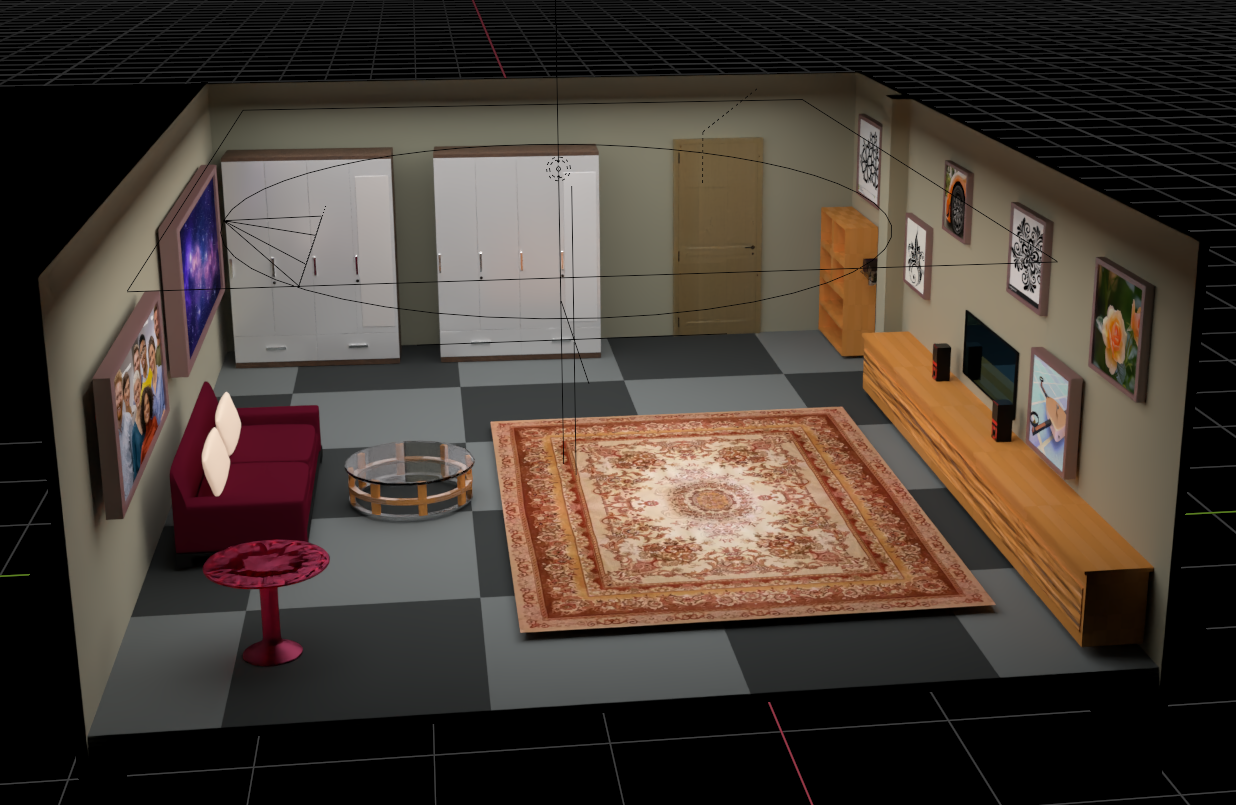
\includegraphics[width=0.9\linewidth]{res/03_research/blender_room/room_layout.png}
    \end{center}
    \caption{Overview of the synthetic room. The ceiling and the nearest wall are
    hidden to give an unobstructed view of the interior, its furniture, and the
    wall-mounted photographs used as dense visual features.}
    \label{fig:room-layout}
\end{figure}

All imagery is produced with Blender's physically based path-tracing renderer,
\emph{Cycles}, configured for GPU compute. The export script enables the available
NVIDIA devices through the OptiX/CUDA back-ends and renders each configured camera
over the full timeline, writing one image per frame. Path tracing rather than a
rasterized preview is used deliberately: it produces physically correct soft
shadows, indirect illumination, and material response. The ground-truth images
therefore contain the kind of view-dependent shading that the spherical-harmonic
appearance model is meant to capture, rather than the flat shading a real-time
engine would give. Because rendering is fully automated through \emph{bpy}, the
entire dataset, every camera and every frame, can be regenerated deterministically
from the scene file, which is what makes the ground truth reproducible.

\newpage

Two camera configurations are exported from the same scene, one for each half of the
static-dynamic decomposition. The static background is reconstructed
from a single camera that traverses a continuous, oscillating trajectory chosen to
maximize spatial coverage of the room while keeping its centre in view. Placing the
geometric centre of the room at the origin, the camera position at frame $t$ is
given by the parametric path
\begin{equation}
    \begin{cases}
        x(t) = r_x \, \sin\!\big(2\pi \tfrac{t}{T}\big) \\
        y(t) = r_y \, \cos\!\big(2\pi \tfrac{t}{T}\big) \\
        z(t) = r_z \, \sin(\omega t)
    \end{cases},
    \label{eq:traj}
\end{equation}
where the symbols are: $t$, the current frame index; $T$, the total number of
frames, so that the normalized time $t/T$ runs over $[0,1]$ and the $xy$-component
completes exactly one revolution; $r_x, r_y, r_z$, the per-axis radii setting how
far the camera swings from the centre along each world axis; and $\omega$, an
angular-frequency factor governing the vertical oscillation. The first two equations
trace an ellipse in the horizontal $xy$-plane (a slow orbit around the room), while
the third superimposes a rapid vertical bob whose frequency $\omega$ is set high
relative to the orbital period. The motivation for this particular path is that
neither a single horizontal orbit nor a single vertical sweep alone yields the
\emph{wide-baseline parallax in all three dimensions} that a full 3D reconstruction
requires. A planar orbit leaves vertical structure poorly constrained, and a single
sweep under-samples the angular dimension. Combining a full azimuthal revolution
with a high-frequency vertical oscillation samples each viewing direction from many
heights and slight positional offsets, approximating a person walking around the
room while raising and lowering the camera. This yields an approximately uniform
distribution of viewpoints that avoids over-fitting the reconstruction to any
densely sampled region.

The dynamic foreground is captured by a rig of $C =
4$ \emph{fixed} cameras placed at the corners of the room, all aimed at the acting
volume at its centre (Figure~\ref{fig:camera-rig}). Each camera is stationary for
the entire capture and records exactly one image per time step. The subject moves,
the cameras do not. The motivation for this seemingly restrictive choice is that it
is precisely what makes a 4D reconstruction well-posed from few cameras.
Across the four cameras, the rig supplies the multi-view parallax needed to
triangulate a 3D cloud at any single instant, the four corners see the subject from
four sufficiently different directions. Across time, the image index $t$ of
every camera gives observation $t$ of frame $t$ of the reconstruction. A single
moving camera, by contrast, observes the moving subject from exactly one direction
at any given instant, so at no instant does it provide the multi-view constraint
needed to fix the subject's 3D shape. It can reconstruct a static room over time but
not a moving subject. The fixed multi-camera rig trades the rich viewpoint coverage
of a moving camera (which it does not need, since the subject supplies the novelty)
for the synchronous multi-view coverage that the dynamic problem does need.

\begin{figure}[!ht]
    \centering
    \begin{tikzpicture}[
  font=\small,
  cambody/.style={draw=black!80, fill=black!75, minimum size=3.2mm, inner sep=0pt},
  frus/.style={draw=blue!60!black, dashed, thick},
  ar/.style={-{Latex[length=2.2mm]}, thick},
]
% --- room footprint (top-down) ----------------------------------------------
\draw[rounded corners=2pt, draw=gray!55!black, thick, fill=gray!6] (-3.6,-3.6) rectangle (3.6,3.6);
\node[gray!55!black, anchor=north east, font=\footnotesize] at (2,3.5) {room ($xy$ floor plan)};
% --- silhouette cones (translucent; overlap darkens toward the subject) ------
\fill[blue!30, opacity=0.16] (-3,-3) -- (-0.75,0.45) -- (0.45,-0.75) -- cycle;
\fill[blue!30, opacity=0.16] ( 3,-3) -- ( 0.75,0.45) -- (-0.45,-0.75) -- cycle;
\fill[blue!30, opacity=0.16] ( 3, 3) -- ( 0.75,-0.45) -- (-0.45,0.75) -- cycle;
\fill[blue!30, opacity=0.16] (-3, 3) -- (-0.75,-0.45) -- (0.45,0.75) -- cycle;
\foreach \x/\y/\name/\lp in {-3/-3/static1/left, 3/-3/static2/right, 3/3/static3/right, -3/3/static4/left}{
  \node[cambody] (c) at (\x,\y) {};
  \node[font=\footnotesize, \lp] at ({\x*1.2},{\y}) {\name};
}
% --- moving subject at the centre (simple figure glyph) ---------------------
\begin{scope}[shift={(0,-0.05)}, draw=red!60!black, thick]
  \fill[red!60!black] (0,0.42) circle (0.16);                 % head
  \draw (0,0.26) -- (0,-0.30);                                % torso
  \draw (-0.28,0.02) -- (0.28,0.02);                          % arms
  \draw (0,-0.30) -- (-0.22,-0.72);                           % left leg
  \draw (0,-0.30) -- ( 0.22,-0.72);                           % right leg
\end{scope}
\node[red!60!black, font=\footnotesize\bfseries, anchor=west] at (0.55,-0.45) {moving subject};
% --- world axes (in-plane x, y) ---------------------------------------------
\begin{scope}[shift={(-3.05,-3.05)}]
  \draw[ar, red!70!black]   (0,0) -- (0.85,0) node[right, font=\scriptsize]{$x$};
  \draw[ar, green!55!black] (0,0) -- (0,0.85) node[above, font=\scriptsize]{$y$};
\end{scope}
% --- annotation -------------------------------------------------------------
\node[blue!55!black, font=\footnotesize] at (0,4.05) {fixed cameras $+$ moving subject $\Rightarrow$ inter-camera parallax};
\end{tikzpicture}
    \caption{Top-down view of the dynamic-capture rig. Four fixed cameras
    (\texttt{static1} to \texttt{static4}) observe a moving subject from the room
    corners. The overlap of their view cones near the subject is the volume in which
    all four silhouettes agree: the region the reconstruction can constrain from
    every side, and the basis of the visual-hull seed of Section~\ref{sec:hull}.}
    \label{fig:camera-rig}
\end{figure}

The decisive methodological choice in the data pipeline is that camera poses are
\textbf{exported directly from Blender rather than estimated from the rendered
images.} An earlier version of this work recovered poses with a Structure-from-Motion
stage that extracted image features, matched them across views, and solved jointly
for poses and a sparse point cloud. That stage was removed for the reason developed
in the Problem Statement. In a dynamic capture, the residual error of pose estimation
is statistically indistinguishable from genuine scene motion. Any pose noise is
therefore silently re-interpreted by the tracker as movement and corrupts the very
quantity being measured. Even in the static case, Structure-from-Motion introduces an
arbitrary global scale and gauge, requires distortion modelling, and can fail
outright in textureless regions. Reading the poses from the source scene eliminates
all of this at the root. The extrinsics are exact  and
the metric scale is the modelled scale of the room. For every rendered frame the exporter records the world matrix of the active camera,
the rigid camera-to-world transform
\begin{equation}
    \mathbf{M}^{\text{c2w}} =
    \begin{bmatrix} \mathbf{R} & \mathbf{c} \\ \mathbf{0}^T & 1 \end{bmatrix}
    \in \mathbb{R}^{4\times4},
    \label{eq:c2w}
\end{equation}
in which the rotation block $\mathbf{R}\in SO(3)$ gives the orientation of the camera
axes in world coordinates and the translation $\mathbf{c}\in\mathbb{R}^3$ is the
optical centre in world coordinates. The inverse, the world-to-camera transform that
the rasterizer consumes, is
\begin{equation}
    \mathbf{M}^{\text{w2c}} = \big(\mathbf{M}^{\text{c2w}}\big)^{-1}
    = \begin{bmatrix} \mathbf{R}^T & -\mathbf{R}^T\mathbf{c} \\ \mathbf{0}^T & 1 \end{bmatrix},
\end{equation}
which maps a world point into the camera frame. For a static camera the matrix in
Eq.~\eqref{eq:c2w} is computed once and reused for all of that camera's frames. For a
moving camera it is re-read on every frame, so that the exported pose always
corresponds exactly to the image that was rendered. The intrinsics follow the ideal pinhole model. Because the imagery is synthetic there
is no lens distortion ($k_1 = k_2 = p_1 = p_2 = 0$), so the undistortion step a real
capture would require is unnecessary, and the mapping from a camera-space point to a
pixel is the linear projection through the intrinsic matrix
\begin{equation}
    \mathbf{K} =
    \begin{bmatrix} f_x & 0 & c_x \\ 0 & f_y & c_y \\ 0 & 0 & 1 \end{bmatrix}.
\end{equation}
Here $f_x, f_y$ are the focal lengths expressed in pixels and $(c_x, c_y)$ is the
principal point, the pixel at which the optical axis pierces the image plane. These
are derived from the physical sensor model of the virtual camera, given a focal
length $f$ in millimetres, a sensor width $s_w$ (the dimension the sensor is fit to
under a horizontal fit), and a rendered resolution of $w \times h$ pixels,
\begin{equation}
    f_x = \frac{f}{s_w}\, w, \qquad f_y = f_x\,\frac{a_x}{a_y},
    \qquad c_x = \frac{w}{2}, \qquad c_y = \frac{h}{2},
    \label{eq:intrinsics}
\end{equation}
where $a_x, a_y$ are the horizontal and vertical pixel aspect ratios (both unity in
this work) and the principal point is fixed at the geometric image centre because the
virtual sensor is centred. The factor $f/s_w$ converts the physical focal length into
a fraction of the sensor width, and multiplying by the pixel width $w$ converts that
fraction into pixels. For compatibility with the Blender / instant-NGP data
convention the exporter also records the horizontal field of view $2\arctan\!\big(w /
2f_x\big)$. But it is the explicit $f_x, f_y, c_x, c_y, w, h$ that the nerfstudio data
parser consumes, since the field-of-view angle alone does not determine the principal
point. Figure \ref{fig:room-mosaic} shows few samples from the generated room-scan dataset for the static background reconstruction.

\begin{figure}[!ht]
    \begin{center}
        \includegraphics[width=1.0\linewidth]{res/03_research/blender_room/room_mosaic.png}
    \end{center}
    \caption{Four representative ground-truth renders from the synthetic dataset,
    illustrating the variation in viewpoint, structural coverage, and lighting
    produced by the camera configurations.}
    \label{fig:room-mosaic}
\end{figure}

\newpage

A recurring source of subtle, hard-to-diagnose errors in multi-view pipelines is the
disagreement between coordinate conventions used by different tools, so the
conventions are stated here explicitly. Blender places the camera's local axes with
$x$ pointing right, $y$ pointing up, and the optical axis along the negative
$z$ direction (an OpenGL-style frame), the matrix of Eq.~\eqref{eq:c2w} is exported
in this frame. Many Structure-from-Motion and computer-vision tools instead use the
OpenCV convention, with $x$ right, $y$ down, and the optical axis along the
positive $z$ direction. The two frames differ by a flip of the $y$ and $z$
axes, $\mathbf{R}_{\text{flip}} = \mathrm{diag}(1,-1,-1)$, as illustrated in
Figure~\ref{fig:coord}. Because the poses here are exported in Blender's convention,
this reconciliation is applied once, deterministically, when the dataset is loaded,
rather than being inferred. Inference would itself be another error source, and the
direct-export pipeline removes it, since there is no ambiguity about which convention
the poses are in.

\begin{figure}[!ht]
    \centering
    \begin{tikzpicture}[
  font=\small,
  ax/.style={-{Latex[length=2.2mm]}, very thick},
  cam/.style={draw=black!75, fill=black!10, thick},
]
% ============================ Blender convention ============================
\begin{scope}
  \node[font=\bfseries] at (0,2.2) {Blender camera};
  \node[cam, trapezium, trapezium left angle=70, trapezium right angle=70,
        minimum width=0.9cm, minimum height=0.5cm, rotate=-90] at (0,0) {};
  \draw[ax, red!70!black]   (0,0) -- (1.4,0)    node[right]{$x$ (right)};
  \draw[ax, green!55!black] (0,0) -- (0,1.4)    node[above]{$y$ (up)};
  \draw[ax, blue!65!black]  (0,0) -- (-1.15,-0.75) node[below left]{$-z$ (look)};
\end{scope}

% ============================ OpenCV convention =============================
\begin{scope}[shift={(6.4,0)}]
  \node[font=\bfseries] at (0,2.2) {OpenCV / SfM camera};
  \node[cam, trapezium, trapezium left angle=70, trapezium right angle=70,
        minimum width=0.9cm, minimum height=0.5cm, rotate=90] at (0,0) {};
  \draw[ax, red!70!black]   (0,0) -- (1.4,0)     node[right]{$x$ (right)};
  \draw[ax, green!55!black] (0,0) -- (0,-1.4)    node[below]{$y$ (down)};
  \draw[ax, blue!65!black]  (0,0) -- (1.15,0.75) node[above right]{$+z$ (look)};
\end{scope}

% ============================ reconciliation ================================
\draw[{Latex[length=2.6mm]}-{Latex[length=2.6mm]}, thick, black!60] (1.9,0.1) -- (4.5,0.1);
\node[align=center, font=\footnotesize, fill=white, inner sep=1pt] at (3.2,0.1)
  {$\mathbf{R}_{\text{flip}}=\mathrm{diag}(1,-1,-1)$\\ reconciled on load};
\end{tikzpicture}

    \caption{Camera coordinate conventions. Blender (left) looks along local $-z$
    with $y$ up; the OpenCV/SfM convention (right) looks along $+z$ with $y$ down.
    The two differ by $\mathbf{R}_{\text{flip}} = \mathrm{diag}(1,-1,-1)$, reconciled
    once at load time.}
    \label{fig:coord}
\end{figure}

Each camera is exported as a self-contained nerfstudio dataset, a folder containing a
\texttt{transforms.json} with the explicit intrinsics of Eq.~\eqref{eq:intrinsics} and
the per-frame poses of Eq.~\eqref{eq:c2w}, alongside an \texttt{images/} directory
holding one zero-padded image per time step. The four fixed cameras therefore form
four sibling folders that share a common frame indexing:
\begin{verbatim}
output/
    static1/  transforms.json  images/{0001..0150}.png
    static2/  transforms.json  images/{0001..0150}.png
    static3/  transforms.json  images/{0001..0150}.png
    static4/  transforms.json  images/{0001..0150}.png
\end{verbatim}
The temporal data parser discovers every camera folder whose name matches the
configured prefix, then \emph{flattens} the per-camera sequences into a single
time-indexed dataset usable by the optimizer. Two consistency conditions are checked
before training begins, and both encode the synchronization assumption the method
depends on. First, every camera must contribute the same number of frames. Second,
the zero-padded filenames must align across cameras so that image $t$ of every camera
genuinely corresponds to the same instant. A missing or mismatched frame is treated
as a fatal error rather than silently skipped, because an asynchronous frame would
appear to the tracker as a sudden, physically impossible jump of the entire subject,
exactly the kind of spurious motion the method cannot and should not try to explain. The four exact poses and the aligned, time-indexed image set are the only
inputs to the reconstruction, no point cloud and no pose estimate are required.

\subsection{Static-Dynamic Scene Decomposition}
\label{sec:decomposition}

The organizing principle introduced in Section~\ref{sec:overview} is now made
precise. Writing $\mathcal{G}_t$ for the set of Gaussians representing the scene at
time $t$, the model assumes the scene decomposes as the disjoint union of a static
and a dynamic component,
\begin{equation}
    \mathcal{G}_t = \mathcal{G}^{\text{static}} \;\sqcup\; \mathcal{G}^{\text{dynamic}}_t,
\end{equation}
subject to the temporal constraints
\begin{equation}
    \forall t:\;\; g_i \in \mathcal{G}^{\text{static}} \Rightarrow \boldsymbol{\mu}_i(t) = \boldsymbol{\mu}_i(0),
    \qquad
    g_i \in \mathcal{G}^{\text{dynamic}}_t \Rightarrow \boldsymbol{\mu}_i(t) = \boldsymbol{\mu}_i(0) + \boldsymbol{\delta}_i(t),
\end{equation}
where the symbol $\sqcup$ denotes a disjoint union (the two sets share no primitive)
and $\boldsymbol{\delta}_i(t) \in \mathbb{R}^3$ is the per-primitive, per-frame
displacement of a dynamic primitive from its rest position. A static
primitive keeps its frame-$0$ position for the whole capture, while a dynamic
primitive is displaced from it by $\boldsymbol{\delta}_i(t)$. The static component is
the rigid scene (walls, floor, ceiling, furniture, stationary objects) and is
reconstructed once as an ordinary Gaussian field. The dynamic component is the moving
subject and is reconstructed per frame.

\subsubsection{Model-Free Foreground Segmentation}
\label{sec:bgsub}

Both the visual-hull seed of Section~\ref{sec:hull} and the silhouette supervision of
Section~\ref{sec:masking} require the moving subject to be presented to the foreground
optimizer \emph{on a black background}. Each recovers the subject's silhouette in a view by
thresholding image brightness, which is only meaningful once everything that is \emph{not}
the subject has been set to black. The foreground branch must therefore be handed images in
which the room has been removed and only the subject remains. The obvious way to obtain them
is to run a learned segmentation network, but that re-introduces precisely the kind of
external, separately-trained dependency the pose pipeline of Section~\ref{sec:data} was at
pains to eliminate. A segmenter must itself be trained, can fail on the thin or deforming
boundaries of a moving subject, and couples the reconstruction's accuracy to a component
that lives outside it. The fixed-camera rig makes a learned segmenter unnecessary. Because every camera is
stationary, the background it observes is identical in every frame, and only the
subject moves. A single photograph of the empty room, taken by each camera before the
subject enters, is therefore a complete model of that camera's background. The subject in
any later frame is then exactly wherever that frame differs from the empty-room photograph.
This is classical background subtraction, and for a static rig under the deterministic
lighting of the synthetic environment (Section~\ref{sec:data}) it is essentially exact. It is
triggered by one convention, the frame indexed $0$ of each camera is reserved for the
empty-room \emph{background plate} $I^{\mathrm{bg}}_c$. When the plate is present the
segmentation runs, when it is absent the images are taken to be already segmented and the step is skipped. Concretely, for camera $c$ and reconstruction frame $t$ the per-pixel change magnitude
against that camera's plate is the mean absolute colour difference,
\begin{equation}
    d_{c,t}(\mathbf{u}) = \tfrac{1}{3}\textstyle\sum_{k} \big| I_{c,t,k}(\mathbf{u}) - I^{\mathrm{bg}}_{c,k}(\mathbf{u}) \big|,
\end{equation}
where the sum runs over the three colour channels $k$ at pixel $\mathbf{u}$, and the
foreground silhouette is its threshold,
\begin{equation}
    \mathcal{S}_{c,t}(\mathbf{u}) = \big[\, d_{c,t}(\mathbf{u}) > \tau_s \,\big],
    \qquad \tau_s = 0.1,
    \label{eq:bgsub}
\end{equation}
with $\tau_s$ a small change threshold and the bracket the Iverson bracket (one where the
predicate holds, zero otherwise). A morphological opening (an erosion followed by a
dilation) removes isolated speckle such as anti-aliasing along edges and the faint flicker
of indirect light on the static surfaces. A final few-pixel dilation keeps the soft
object boundary from being clipped. The image actually handed to the optimizer is the
original frame with everything outside the silhouette set to black,
\begin{equation}
    \tilde I_{c,t} = I_{c,t} \odot \mathcal{S}_{c,t},
    \label{eq:segmented}
\end{equation}
so that every unchanged pixel becomes exactly the black background the rest of the foreground
pipeline assumes (Figure~\ref{fig:bgsub}). The plate $I^{\mathrm{bg}}_c$ has done its work
once the silhouettes are computed and is not itself a reconstruction frame. With a
plate plus $F$ subject frames the reconstruction still has $F$ frames, and the step schedule
of Section~\ref{sec:temporal} is sized accordingly.

\begin{figure}[!ht]
    \centering
    \resizebox{0.96\textwidth}{!}{\begin{tikzpicture}[
  font=\small,
  imgf/.style={draw=black!55, thick, rounded corners=1.5pt, minimum width=2.4cm, minimum height=1.5cm, inner sep=0pt},
  lbl/.style={font=\footnotesize, align=center},
  ar/.style={-{Latex[length=2.4mm]}, thick, draw=black!70},
  furn/.style={fill=gray!45},
  obj/.style={fill=red!65!black, draw=red!40!black, very thin},
  combine/.style={circle, draw=black!70, thick, inner sep=1.2pt, font=\footnotesize},
]
% ---------- input 1: empty-room background plate (frame 0) ----------
\node[imgf, fill=blue!5] (plate) at (0,1.25) {};
\begin{scope}
  \clip (plate.south west) rectangle (plate.north east);
  \begin{scope}[shift={(plate.center)}]
    \fill[furn] (-0.95,-0.45) rectangle (-0.45,0.05);
    \fill[furn] (0.45,-0.55) rectangle (0.95,0.2);
  \end{scope}
\end{scope}
\node[lbl, above=1pt of plate] {empty-room plate $I^{\mathrm{bg}}_c$\\ (frame $0$)};

% ---------- input 2: object frame ----------
\node[imgf, fill=blue!5] (frame) at (0,-1.25) {};
\begin{scope}
  \clip (frame.south west) rectangle (frame.north east);
  \begin{scope}[shift={(frame.center)}]
    \fill[furn] (-0.95,-0.45) rectangle (-0.45,0.05);
    \fill[furn] (0.45,-0.55) rectangle (0.95,0.2);
    \fill[gray!35] (-0.05,-0.62) ellipse (0.45 and 0.1); % faint cast shadow
    \fill[obj] plot[smooth cycle, tension=0.7] coordinates {(0.07,0.5) (0.35,0.1) (0.28,-0.4) (-0.05,-0.55) (-0.34,-0.18) (-0.28,0.32)};
  \end{scope}
\end{scope}
\node[lbl, below=1pt of frame] {object frame $I_{c,t}$};

% ---------- subtraction ----------
\node[combine] (minus) at (2.2,0) {$-$};
\draw[ar] (plate.east) to[out=0,in=120]  (minus);
\draw[ar] (frame.east) to[out=0,in=-120] (minus);

% ---------- change magnitude ----------
\node[imgf, fill=black!90] (diff) at (5.0,0) {};
\begin{scope}
  \clip (diff.south west) rectangle (diff.north east);
  \begin{scope}[shift={(diff.center)}]
    \fill[gray!22] (-0.05,-0.62) ellipse (0.45 and 0.1); % residual shadow change
    \fill[white] plot[smooth cycle, tension=0.7] coordinates {(0.07,0.5) (0.35,0.1) (0.28,-0.4) (-0.05,-0.55) (-0.34,-0.18) (-0.28,0.32)};
  \end{scope}
\end{scope}
\node[lbl, below=2pt of diff] {change magnitude\\ $d_{c,t}=\tfrac13\sum_k|I_{c,t,k}-I^{\mathrm{bg}}_{c,k}|$};
\draw[ar] (minus) -- (diff);

% ---------- segmented input ----------
\node[imgf, fill=black!90] (seg) at (9.4,0) {};
\begin{scope}
  \clip (seg.south west) rectangle (seg.north east);
  \begin{scope}[shift={(seg.center)}]
    \fill[obj] plot[smooth cycle, tension=0.7] coordinates {(0.07,0.5) (0.35,0.1) (0.28,-0.4) (-0.05,-0.55) (-0.34,-0.18) (-0.28,0.32)};
  \end{scope}
\end{scope}
\node[lbl, below=2pt of seg] {segmented input\\ $\tilde I_{c,t}=I_{c,t}\odot\mathcal{S}_{c,t}$};
\draw[ar] (diff) -- (seg) node[midway, above, lbl] {threshold $\tau_s$,\\ open\,/\,dilate,\\ black out};
\end{tikzpicture}
}
    \caption{Model-free foreground segmentation by background subtraction. Each fixed camera
    contributes an empty-room background plate (frame $0$), subtracting it from a later
    frame and thresholding the change magnitude (Eq.~\eqref{eq:bgsub}) yields the subject's
    silhouette with no learned model. Everything outside the silhouette is set to black
    (Eq.~\eqref{eq:segmented}), producing exactly the on-black input the visual hull and the
    silhouette loss expect. The faint cast shadow that leaks into a single view is removed by
    the multi-view hull intersection.}
    \label{fig:bgsub}
\end{figure}

\subsubsection{Background gradient and filtering}

Background subtraction attributes
any image change to the subject, including the soft shadow it casts and the indirect
light it bounces onto nearby static surfaces, so a single camera's silhouette can bleed a
little beyond the true object. Two mechanisms keep this minimized. The morphological opening
removes the thin, low-contrast shadow fringe directly. More importantly, the per-view
silhouettes are never trusted on their own. The visual hull of Section~\ref{sec:hull} retains
only voxels that fall inside the foreground of every camera. A cast shadow on the
floor that one camera registers as foreground is not seen as foreground by the others, so it
is carved away by the same silhouette intersection that builds the seed. The threshold
$\tau_s$ can be raised if low-contrast leakage persists. The background subtraction separates foreground
from background in image space. The partition of the reconstructed primitives
into the static set $\mathcal{G}^{\text{static}}$ and the dynamic set
$\mathcal{G}^{\text{dynamic}}_t$ then follows from the optimization itself, with no further
labelling. The mechanism is visible directly in the gradient (Figure~\ref{fig:decomp}). A
primitive on a stationary surface projects to a pixel whose value does not change from frame
to frame (except briefly when the subject occludes it), so its expected positional gradient
is essentially zero,
\begin{equation}
    g_i \in \mathcal{G}^{\text{static}}:\quad \mathbb{E}\!\big[\nabla_{\boldsymbol{\mu}_i}\mathcal{L}_t\big] \approx \mathbf{0},
\end{equation}
and it remains numerically stationary. A primitive on the moving subject projects to a
pixel that changes every frame, so its expected gradient has a well-defined direction
opposing the local error, driving it along the subject's motion,
\begin{equation}
    g_i \in \mathcal{G}^{\text{dynamic}}_t:\quad \mathbb{E}\!\big[\nabla_{\boldsymbol{\mu}_i}\mathcal{L}_t\big] \;\propto\; -\,\mathbf{v}^{(i)}_t.
\end{equation}
No \emph{learned} segmenter is needed anywhere in this chain, a per-pixel image difference
supplies the foreground silhouette, and the loss landscape itself partitions the
reconstructed cloud. A useful empirical consequence is that the partition can also be
read off after the fact by thresholding each primitive's cumulative displacement,
$D_i = \sum_{t} \|\boldsymbol{\mu}_i(t) - \boldsymbol{\mu}_i(t-1)\|_2$. Its distribution
over the cloud is strongly bimodal, with a tight peak near zero for the stationary parts
and a long tail for the moving subject, so a single threshold cleanly recovers the moving
set, again without any learned segmentation having been performed.

\begin{figure}[!ht]
    \centering
    \resizebox{0.9\textwidth}{!}{\begin{tikzpicture}[
  font=\small,
  gpt/.style={circle, inner sep=1.6pt},
  grad/.style={-{Latex[length=2.4mm]}, very thick},
]
% --- wall (static) region ---------------------------------------------------
\draw[fill=gray!10, draw=gray!55!black, thick] (-0.4,-1.6) rectangle (3.2,1.8);
\node[gray!55!black, anchor=north west, font=\footnotesize] at (-0.3,1.7) {static wall};
\foreach \x/\y in {0.3/1.2, 1.0/0.4, 1.7/1.1, 2.4/-0.3, 0.7/-1.0, 2.0/0.7}{
  \node[gpt, fill=gray!55!black] at (\x,\y) {};
}
\node[align=center, font=\footnotesize, fill=white, inner sep=1pt] at (1.4,-2.2)
  {$\mathbb{E}[\nabla_{\boldsymbol{\mu}_i}\mathcal{L}]\approx\mathbf{0}$\\ primitive stays};

% --- moving subject (dynamic) region ----------------------------------------
\begin{scope}[shift={(6.4,0)}]
  \draw[fill=red!8, draw=red!55!black, thick] (-1.0,-1.6) rectangle (2,1.8);
  \node[red!55!black, anchor=north west, font=\footnotesize] at (-0.95,1.7) {moving subject};
  % a few primitives with motion arrows
  \foreach \x/\y in {-0.4/0.9, 0.2/0.2, 0.6/1.0, -0.2/-0.6, 0.4/-1.0}{
    \node[gpt, fill=red!65!black] (g) at (\x,\y) {};
    \draw[grad, red!65!black] (\x,\y) -- ($(\x,\y)+(0.6,-0.18)$);
  }
  \node[align=center, font=\footnotesize, fill=white, inner sep=1pt] at (0.2,-2.2)
    {$\mathbb{E}[\nabla_{\boldsymbol{\mu}_i}\mathcal{L}]\propto-\mathbf{v}^{(i)}_t$\\ primitive moves};
\end{scope}

% --- shared label -----------------------------------------------------------
\node[font=\footnotesize\bfseries] at (4.0,2.5) {emergent partition (no explicit mask)};
\end{tikzpicture}
}
    \caption{The emergent static-dynamic partition. A primitive on the static wall
    receives a near-zero expected positional gradient and stays put. A primitive on
    the moving subject receives a gradient aligned with $-\mathbf{v}^{(i)}_t$ and
    migrates. The partition is a by-product of the optimization rather than an input
    to it.}
    \label{fig:decomp}
\end{figure}

The two components are reconstructed independently and recombined only at render time
(Section~\ref{sec:merge}). During the optimization of the foreground, the background
is not present at all, the subject is fit against the black background produced by the
segmentation of Eq.~\eqref{eq:segmented}, so the two components never compete for the same
pixels and never interfere. This separation is
what allows the foreground method to make the aggressive count- and colour-freezing
assumptions of the next section without those assumptions ever being applied to the
much larger and structurally different background.

\subsection{Reconstructing the Temporal Gaussian Field}
\label{sec:temporal}

\begin{algorithm}[!b]
\SetAlgoLined
\KwIn{aligned multi-view frames $\{I_{c,t}\}$, camera poses $\{\mathbf{M}_c\}$,
      initial budget $N_0$, tracking budget $N_t$, frame count $F$}
\KwOut{per-frame Gaussian clouds $\{\mathcal{G}_t\}_{t=0}^{F-1}$}
$\mathcal{G} \gets \textsc{CarveVisualHull}(\{I_{c,0}\}, \{\mathbf{M}_c\})$ \tcp*{seed inside the object (Alg.~\ref{alg:carve})}
$\boldsymbol{\mu}_{-1}, \boldsymbol{\mu}_{-2} \gets \varnothing$ \tcp*{velocity history}
\For{$t \gets 0$ \KwTo $F-1$}{
    point every camera at its frame-$t$ image\;
    \eIf{$t = 0$}{
        $B \gets N_0$; enable densification \& pruning\;
    }{
        \If{$t \ge 2$}{$\boldsymbol{\mu} \gets \boldsymbol{\mu} + (\boldsymbol{\mu}_{-1} - \boldsymbol{\mu}_{-2})$ \tcp*{velocity prediction, Eq.~\eqref{eq:velocity}}}
        $\mathcal{G} \gets \textsc{SnapStraysToHull}(\mathcal{G}, \{I_{c,t}\})$ \tcp*{frustum clamp (Alg.~\ref{alg:snap})}
        $B \gets N_t$; disable densification; colours frozen\;
    }
    \For{step $\gets 1$ \KwTo $B$}{
        sample a camera $c$; render $\hat I_{c,t}$ via Eq.~\eqref{eq:alphablend}\;
        $\mathcal{L} \gets \mathcal{L}_{\text{photo}} + \mathcal{L}_{\text{sil}}$ on the object mask\;
        backpropagate; take one Adam step on the trainable parameters $\Theta_{\text{track}}$\;
    }
    \If{$t = 0$}{freeze the primitive count and the SH colours \tcp*{constant topology hereafter}}
    $\mathcal{G}_t \gets \mathcal{G}$; \quad $\boldsymbol{\mu}_{-2}\gets\boldsymbol{\mu}_{-1}$; \quad $\boldsymbol{\mu}_{-1}\gets\boldsymbol{\mu}$\;
}
\caption{Temporal Gaussian fitting (\texttt{temporal-splatfacto}).}
\label{alg:temporal}
\end{algorithm}

The dynamic foreground is reconstructed by \texttt{temporal-splatfacto}, whose
complete procedure is given in Algorithm~\ref{alg:temporal}. The remainder of this
section explains and motivates each of its parts in turn, the visual-hull seed
(line~1), the single monotonic step schedule that interleaves an initial block with
one tracking block per frame (the loop structure), the constant-count, frozen-colour
tracking regime (lines~9 to 12), and the velocity prediction and frustum snap applied
at each frame transition (lines~6 to 8, detailed in Section~\ref{sec:velocity}). The
defining feature of the procedure is that it is not a loop of independent
reconstructions but a single, continuous optimization whose behaviour changes as the
global step crosses frame boundaries. Concretely, training is a single, monotonically increasing sequence of optimizer
steps, partitioned into one initial block that reconstructs frame~$0$ and one
fixed-size tracking block per subsequent frame. The active frame is a pure
function of the global step $k$, so the data parser, model, and trainer all agree on
which frame is current without sharing any mutable state. Given $N_0$ initial
iterations and $N_t$ tracking iterations over $F$ frames, the step-to-frame map is
\begin{equation}
    \mathrm{frame}(k) =
    \begin{cases}
        0, & k < N_0, \\[2pt]
        \min\!\Big(1 + \big\lfloor \tfrac{k - N_0}{N_t} \big\rfloor,\; F-1\Big), & k \ge N_0,
    \end{cases}
    \label{eq:frameofstep}
\end{equation}
and, consequently, the total number of steps is \emph{determined} by the frame count
rather than configured by hand,
\begin{equation}
    K_{\text{total}} = N_0 + (F-1)\,N_t .
    \label{eq:ktotal}
\end{equation}
The schedule is illustrated in Figure~\ref{fig:schedule}.

\begin{figure}[!ht]
    \centering
    \resizebox{0.95\textwidth}{!}{\begin{tikzpicture}[
  font=\small,
  brace/.style={decorate, decoration={brace, amplitude=5pt, raise=3pt}, thick},
  trans/.style={-{Latex[length=2.0mm]}, thick, red!65!black},
]
% --- frame-0 (initial) block ------------------------------------------------
\fill[blue!22, draw=blue!60!black, thick] (0,0) rectangle (5,0.9);
\node[align=center] at (2.5,0.45) {\textbf{frame 0}\\ \footnotesize initial fit};

% --- tracking blocks --------------------------------------------------------
\foreach \i/\xa in {1/5, 2/6.3, 3/7.6, 4/8.9, 5/10.2}{
  \fill[green!16, draw=green!55!black, thick] (\xa,0) rectangle ($(\xa,0)+(1.3,0.9)$);
  \node[font=\footnotesize] at ($(\xa,0)+(0.65,0.45)$) {$\;t{=}\i$};
}
\node[font=\footnotesize] at (12.1,0.45) {$\cdots$};
\fill[green!16, draw=green!55!black, thick] (12.4,0) rectangle (13.7,0.9);
\node[font=\footnotesize] at (13.05,0.45) {$t{=}F{-}1$};

% --- step axis --------------------------------------------------------------
\draw[-{Latex[length=2mm]}, thick] (-0.1,-0.35) -- (14.0,-0.35) node[right, font=\footnotesize] {step};
\foreach \x/\lab in {0/0, 5/$N_0$, 6.3/{$N_0{+}N_t$}}{
  \draw (\x,-0.27) -- (\x,-0.43);
}
\node[font=\scriptsize, anchor=north] at (0,-0.5)   {$0$};
\node[font=\scriptsize, anchor=north east] at (5,-0.5)   {$N_0$};
\node[font=\scriptsize, anchor=north east] at (6.3,-0.5){$N_0{+}N_t$};

% --- braces -----------------------------------------------------------------
\draw[brace] (0,0.9) -- (5,0.9) node[midway, above=7pt, align=center, font=\footnotesize]
  {densification on\\ count fixed at step $N_0$};
\draw[brace] (5,0.9) -- (13.7,0.9) node[midway, above=7pt, align=center, font=\footnotesize]
  {tracking: count \& colour frozen\\ $N_t$ steps each};

% --- frame transitions: velocity + snap -------------------------------------
\foreach \x in {5,6.3,7.6,8.9,10.2,12.4}{
  \draw[trans] (\x,-1.25) -- (\x,-0.05);
}
\node[red!65!black, font=\footnotesize, anchor=north, align=center] at (7.5,-1.3)
  {at each transition: velocity prediction $+$ frustum snap};
\end{tikzpicture}
}
    \caption{The training schedule. Frame~$0$ receives a large budget $N_0$ with
    densification active. The primitive count is frozen at step $N_0$. Each subsequent
    frame receives $N_t$ tracking steps with the count and colour held constant. Every
    frame transition applies a velocity prediction followed by a frustum snap
    (Section~\ref{sec:velocity}).}
    \label{fig:schedule}
\end{figure}

Expressing the whole capture
as one continuous step sequence, rather than as $F$ separate training runs, is what
lets the method inherit the host framework's machinery unchanged, namely a single
optimizer with per-parameter state, the standard checkpointing, and the live viewer.
It also makes the schedule self-describing, from the global step alone, every
component can compute the current frame (Eq.~\eqref{eq:frameofstep}), whether this is
the first or last step of that frame (used to trigger per-frame setup and saving), and
the local step within the frame (used to schedule learning rates). The price is only
that the optimizer's momentum carries across frame boundaries, which is in fact
desirable, a smoothly moving subject induces smoothly varying gradients, so momentum
accumulated on one frame is a reasonable prior for the next.

\subsubsection{Visual-Hull Initialization}
\label{sec:hull}

3D Gaussian Splatting is notoriously sensitive to
initialization; a poor seed leads to floaters, a prolonged densification phase, or
outright divergence. The standard remedy is to seed from a Structure-from-Motion
point cloud, but that is exactly the dependency this work removed. Two seed-free
alternatives exist: a random cloud in a bounding box, or a geometry-aware seed derived
from the images. A random box wastes most of its primitives outside the object, which
the optimizer must then spend iterations culling, and it provides no colour prior. The
key observation here is that the subject is rendered against a black background, so the
object's \emph{silhouette} in each camera is trivially available by thresholding
brightness. The intersection of the silhouette cones from several cameras, the
classical \emph{visual hull}, is a tight, bounded volume that already hugs the object
from every side. Seeding inside this hull places primitives where they are needed from
the very first iteration, with no stray background primitives to cull later, and is
the geometry-aware initialization the method uses (Algorithm~\ref{alg:carve}).

\begin{algorithm}[H]
\SetAlgoLined
\KwIn{frame-$0$ images $\{I_c\}_{c=1}^{C}$, poses $\{\mathbf{M}_c\}$, grid resolution
      $R$, brightness threshold $\tau_b$, view fraction $\rho$}
\KwOut{seed points $\mathcal{H}$ with colours}
build a voxel grid of $R^3$ centres over a cube spanning the cameras\;
\ForEach{camera $c$}{
    $\mathcal{M}_c \gets [\,\bar I_c > \tau_b\,]$ \tcp*{brightness foreground mask}
    optionally dilate $\mathcal{M}_c$ by a few pixels\;
}
\ForEach{voxel centre $\mathbf{x}$}{
    $n(\mathbf{x}) \gets \sum_{c} \mathcal{M}_c\big(\pi(\mathbf{K}_c\mathbf{M}_c^{\text{w2c}}\mathbf{x})\big)$ \tcp*{\# cameras seeing it as foreground}
}
$\mathcal{H} \gets \{\mathbf{x} : n(\mathbf{x}) \ge \rho\,C\}$ \tcp*{silhouette intersection}
colour each $\mathbf{x}\in\mathcal{H}$ by its mean projected image sample\;
subsample $\mathcal{H}$ to the point budget if necessary\;
\caption{Visual-hull carving (\textsc{CarveVisualHull}).}
\label{alg:carve}
\end{algorithm}

A voxel grid of resolution $R^3$ (default $R = 192$) is laid over a cube centred on
the cameras. Each frame-$0$ image is converted to a foreground mask by thresholding
its per-pixel brightness,
\begin{equation}
    \mathcal{M}_c(\mathbf{u}) = \big[\,\bar I_c(\mathbf{u}) > \tau_b\,\big],
    \qquad \bar I_c(\mathbf{u}) = \tfrac{1}{3}\textstyle\sum_{k} I_{c,k}(\mathbf{u}),
\end{equation}
where $\bar I_c(\mathbf{u})$ is the mean of the three colour channels at pixel
$\mathbf{u}$, $\tau_b = 0.05$ is the brightness threshold separating the lit subject
from the black background, and the bracket is the Iverson bracket (one when the
predicate holds, zero otherwise). The mask is optionally dilated by a few pixels to
be forgiving at silhouette edges, where antialiasing makes the boundary gradual. Each
voxel centre $\mathbf{x}$ is projected into every camera through its world-to-camera
transform and intrinsics, $\mathbf{u}_c = \pi\!\big(\mathbf{K}_c
\mathbf{M}_c^{\text{w2c}} \mathbf{x}\big)$ where $\pi$ is the perspective divide, and
a voxel is retained when it lands in the foreground mask of at least a fraction $\rho$
of the cameras:
\begin{equation}
    \mathcal{H} = \Big\{\, \mathbf{x} \;:\; \textstyle\sum_{c=1}^{C} \mathcal{M}_c\big(\mathbf{u}_c(\mathbf{x})\big) \;\ge\; \rho\, C \,\Big\}.
    \label{eq:hull}
\end{equation}
With $\rho = 1$ this is the strict intersection of all four silhouette cones
(Figure~\ref{fig:visual-hull}). A slightly smaller $\rho$ keeps a voxel that is
foreground in, say, three of four cameras, which tolerates mask noise and partial
self-occlusion at the cost of a slightly looser hull. The surviving voxels seed the
Gaussians through nerfstudio's standard seed-point interface, each coloured by the
mean of its projected image samples via Eq.~\eqref{eq:sh2rgb} and subsampled to a
budget if there are too many. Because $\mathcal{H}$ is an \emph{intersection} of exact
silhouette cones rather than a loose bounding box, it bounds the object volume
directly. This is precisely the property that makes it a far better seed than a random
cube, and the reason the hull is preferred over a ``large box, then prune'' strategy
that would spend many early iterations discarding primitives that the hull never
creates.

\begin{figure}[!ht]
    \centering
    \begin{tikzpicture}[
  font=\small,
  cambody/.style={draw=black!80, fill=black!75, minimum size=3mm, inner sep=0pt},
  cone/.style={fill=blue!35, opacity=0.18},
  edge/.style={draw=blue!55!black, very thin, dashed},
  hull/.style={fill=orange!80!red, opacity=0.55},
]
% cameras and tangent-ray endpoints (rays are tangent to the object border)
\coordinate (c1) at (-4,-2.2);  \coordinate (c2) at (4,-2.2);  \coordinate (c3) at (0,3.3);
\coordinate (c1a) at (2.650,-0.015); \coordinate (c1b) at (1.373,2.287);
\coordinate (c2a) at (-1.395,2.261); \coordinate (c2b) at (-2.644,0.004);
\coordinate (c3a) at (-1.687,-3.494); \coordinate (c3b) at (1.650,-3.503);

% --- silhouette cones -------------------------------------------------------
\fill[cone] (c1) -- (c1a) -- (c1b) -- cycle;
\fill[cone] (c2) -- (c2a) -- (c2b) -- cycle;
\fill[cone] (c3) -- (c3a) -- (c3b) -- cycle;

% --- triple intersection = carved visual hull (exact, via nested clipping) --
\begin{scope}
  \clip (c1) -- (c1a) -- (c1b) -- cycle;
  \clip (c2) -- (c2a) -- (c2b) -- cycle;
  \clip (c3) -- (c3a) -- (c3b) -- cycle;
  \fill[hull] (-6,-5) rectangle (6,5);
\end{scope}

% --- tangent beam edges -----------------------------------------------------
\draw[edge] (c1) -- (c1a); \draw[edge] (c1) -- (c1b);
\draw[edge] (c2) -- (c2a); \draw[edge] (c2) -- (c2b);
\draw[edge] (c3) -- (c3a); \draw[edge] (c3) -- (c3b);

% --- the true object (ground-truth silhouette) ------------------------------
\fill[red!55!black, opacity=0.85]
  plot[smooth cycle, tension=0.8] coordinates {(0,0.9) (0.7,0.4) (0.55,-0.5) (0,-0.85) (-0.6,-0.45) (-0.7,0.45)};
\node[white, font=\footnotesize\bfseries] at (0,0) {object};

% --- cameras ----------------------------------------------------------------
\node[cambody] at (c1) {}; \node[font=\footnotesize, left] at (-4.1,-2.2) {cam $1$};
\node[cambody] at (c2) {}; \node[font=\footnotesize, right] at (4.1,-2.2) {cam $2$};
\node[cambody] at (c3) {}; \node[font=\footnotesize, above] at (0,3.45) {cam $3$};

% --- annotations ------------------------------------------------------------
\node[blue!55!black, font=\footnotesize, anchor=west] at (2.2,1.6) {silhouette cone};
\draw[-{Latex[length=1.8mm]}, blue!55!black] (2.15,1.6) to[out=180,in=40] (1.15,1.15);
\node[orange!70!red, font=\footnotesize\bfseries, anchor=west] at (2.5,-0.5) {carved hull};
\draw[-{Latex[length=1.8mm]}, orange!70!red] (2.5,-0.5) to[out=180,in=-40] (0.85,-0.75);
\node[align=center, font=\footnotesize\bfseries, fill=white, inner sep=1pt] at (0,-2.9)
  {carved visual hull $=\ \bigcap_c\,$cone$_c\ \supseteq\ $object};
\end{tikzpicture}
    \caption{Visual-hull carving (shown in 2D for three cameras). Each camera
    contributes a silhouette cone; the carved hull is their intersection, a tight
    superset of the object. The translucent overlap darkens toward the centre, where
    all cones agree.}
    \label{fig:visual-hull}
\end{figure}

\subsubsection{Frame 0: Dense Reconstruction}
\label{sec:frame0}

The first frame is reconstructed by the full Gaussian-Splatting optimizer, with
adaptive density control active, for $N_0$ iterations starting from the hull seed.
This stage plays two roles. The obvious one is to produce a high-quality
reconstruction of the subject in its frame-$0$ pose. The less obvious but more
important one is that it \emph{fixes the primitive count for the rest of the video}:
densification and pruning are hard-stopped at step $N_0$, after which $|\mathcal{G}_t|
= |\mathcal{G}_0|$ for all $t \ge 0$. Densification must be allowed here, because the
hull seed is only a coarse volumetric occupancy and the optimizer needs the freedom
to add primitives where fine detail demands them and to remove primitives the hull
over-included. But it must also be stopped cleanly, because every later frame relies
on the count being constant. The photometric objective is the standard
Gaussian-Splatting loss, a convex combination of an $L_1$ term and a
structural-similarity term,
\begin{equation}
    \mathcal{L}_{\text{photo}} = (1 - \lambda)\,\mathcal{L}_1(\hat I, I)
    + \lambda \big(1 - \mathrm{SSIM}(\hat I, I)\big), \qquad \lambda = 0.2,
    \label{eq:photo}
\end{equation}
where $\mathcal{L}_1(\hat I, I) = \frac{1}{|\Omega|}\sum_{\mathbf{p}\in\Omega}
\|\hat I(\mathbf{p}) - I(\mathbf{p})\|_1$ is the mean absolute pixel error over the
image domain $\Omega$, $\mathrm{SSIM}$ is the structural-similarity index comparing
local means, variances, and covariance of the two images through a small Gaussian
window, and $\lambda = 0.2$ balances the two. The $L_1$ term drives pixel-accurate
colour, while the SSIM term enforces local structural agreement and prevents the
optimizer from smearing a few oversized primitives across the image. As detailed in
Section~\ref{sec:masking}, this loss is in fact restricted to the object region; the
training background is black so that empty image regions cost nothing. At the end of
this stage the cloud is a dense, well-localized reconstruction of the subject with a
primitive count that will never change again.

\subsubsection{Tracking Frames}
\label{sec:tracking}

Each subsequent frame is reconstructed by re-running the optimizer against the
\emph{same} primitives for $N_t$ steps, under three constraints that together turn the
problem from reconstruction into tracking. The constraints are not independent
conveniences; each addresses a specific failure mode of unconstrained per-frame
fitting.

\textbf{Constant count (motivation: correspondence).} Densification and pruning are
disabled and the periodic opacity reset is skipped, so the primitive set is conserved
exactly across the frame. The motivation is correspondence: only if the count is fixed
and no primitive is created or destroyed does the index $i$ refer to the same physical
feature in frame $t$ as in frame $t-1$. That one-to-one correspondence is what makes
velocity estimation (Section~\ref{sec:velocity}), trajectory analysis, and the
per-attribute temporal compression (Section~\ref{sec:compression}) well-defined. A
varying count would break all three. Skipping opacity reset matters for the same
reason: the primitives are already well placed, and resetting their opacity would
discard hard-won information and inject a transient artifact at every frame boundary.

\textbf{Frozen colour (motivation: motion, not repainting).} The
spherical-harmonic coefficients, both the diffuse term $\mathrm{SH}^{(0)}$ and all
higher bands $\mathrm{SH}^{(1..L)}$, are frozen after frame~$0$: their learning
rates are set to zero and their gradient tracking is disabled. The trainable parameter
set during tracking is therefore restricted to geometry and opacity,
\begin{equation}
    \Theta_{\text{track}} = \{\boldsymbol{\mu}_i, \mathbf{s}_i, \mathbf{q}_i, \tilde\sigma_i\}_{i=1}^{N},
    \qquad
    \Theta_{\text{frozen}} = \{\mathrm{SH}^{(0)}_i, \mathrm{SH}^{(1..L)}_i\}_{i=1}^{N},
    \label{eq:trackparams}
\end{equation}
so that for every tracking step the frozen parameters satisfy
$\boldsymbol{\theta}_t = \boldsymbol{\theta}_0$ while the trainable ones follow the
usual gradient update. The motivation is the appearance-motion entanglement of
problem~2. If the optimizer were free to edit colour during tracking, the cheapest way
to lower the loss when the subject moves would often be to \emph{repaint} a stationary
primitive in the new colour, leaving it geometrically wrong but photometrically
correct for that frame. Freezing colour removes that option entirely. With appearance
and population both fixed, the only remaining way to reduce the loss is to \emph{move
and reshape} the primitives, so tracking is forced to align them to the subject's
actual motion. This was verified empirically: across frames the colour tensors are
bit-identical while the means continue to move, confirming that no appearance editing
is occurring. Opacity is deliberately left trainable, for reasons taken up in
Section~\ref{sec:masking}.

\textbf{Per-phase learning rate (motivation: sustained mobility).} The positional
learning rate is scheduled differently in the two phases. During frame~$0$ it follows
the usual exponential decay from $\eta_{\text{init}}$ to $\eta_{\text{final}}$, which
is appropriate for converging a single static reconstruction. During tracking it is
held \emph{constant} at $\eta_{\text{track}}$. The motivation is that a single global
decay schedule, of the kind a static run uses, would shrink the learning rate toward
zero by the late frames and effectively freeze the motion just when the subject is
still moving. The reconstruction would lock up partway through the sequence. A
constant tracking rate keeps every frame, early or late, equally able to follow the
motion. The scale, rotation, and opacity learning rates are likewise kept at their
tracking values, and the image resolution is held at full scale for every frame so
that all frames are fit under identical conditions.

The tracking budget $N_t$ is set to a small fraction of $N_0$. This is only
affordable because of the velocity prediction of the next section, which ensures that
each tracking frame begins already close to its solution. The budget therefore has to
cover only the small residual rather than the full motion arc.

\subsubsection{Foreground Masking and Silhouette Supervision}
\label{sec:masking}

\textbf{The failure mode.} A subtle but destructive problem appears if the loss is
computed naively over the entire image. With a black background, a stationary black
region is matched at essentially zero cost regardless of what the primitives do
nearby, so there is \emph{no force pinning primitives to the silhouette}. Worse, a
bright primitive that drifts a little into the background renders brightly on black
and incurs a large error there. The cheapest way for the optimizer to reduce that
error is not to move it back but to drive its opacity to near zero. It then becomes an
invisible ``dead'' primitive that no longer contributes to any image. Yet the
per-frame velocity prediction (Section~\ref{sec:velocity}) keeps pushing it, so it
accumulates in empty space. Over a sequence the foreground slowly erodes as primitives
leak away, while faint background splats proliferate. The naive full-image loss thus
not only fails to prevent drift, it actively rewards it.

\textbf{The fix: mask the loss and supervise the silhouette.} The remedy is to
restrict the photometric loss to the object and to add an explicit constraint on the
rendered silhouette. Let $\mathcal{M}$ be the brightness mask of the ground-truth
frame (the same construction as in the hull carving) and let $\hat A$ be the rendered
\emph{accumulation} image, the per-pixel sum of alpha contributions, which is the
rendered opacity or coverage at that pixel. The photometric loss of
Eq.~\eqref{eq:photo} is masked to the object,
\begin{equation}
    \mathcal{L}_{\text{photo}} = (1-\lambda)\,\big\| (\hat I - I)\odot \mathcal{M} \big\|_1
    + \lambda\,\big(1 - \mathrm{SSIM}(\hat I \odot \mathcal{M},\, I \odot \mathcal{M})\big),
\end{equation}
where $\odot$ is the element-wise (Hadamard) product, so that only object pixels
contribute. An explicit silhouette term then pushes the rendered opacity to zero
clearly outside the object and gently toward one inside it,
\begin{equation}
    \mathcal{L}_{\text{sil}}
    = \lambda_{\text{out}} \big\| \hat A \odot (1 - \mathcal{M}^{+}) \big\|_1
    + \lambda_{\text{in}} \big\| (1 - \hat A) \odot \mathcal{M}^{-} \big\|_1 ,
    \label{eq:sil}
\end{equation}
where $\mathcal{M}^{+}$ is the mask dilated by a few pixels (its morphological
expansion) and $\mathcal{M}^{-}$ its erosion (its morphological contraction). The
first term penalizes any rendered opacity in the region clearly outside the object,
$1 - \mathcal{M}^{+}$, directly punishing a primitive that strays into the background.
The second gently encourages full opacity in the eroded object core,
$\mathcal{M}^{-}$, keeping the subject solid. The band between the erosion and the
dilation, $\mathcal{M}^{+}\setminus\mathcal{M}^{-}$, is a deliberate ``don't-care''
zone around the true boundary in which opacity is neither pushed to zero nor to one,
so that the soft tails of primitives at the genuine silhouette edge are not fought.
The total objective is $\mathcal{L} = \mathcal{L}_{\text{photo}} +
\mathcal{L}_{\text{sil}}$, with default weights $\lambda_{\text{out}} = 1.0$ and
$\lambda_{\text{in}} = 0.1$. The outside term is weighted an order of magnitude more
strongly than the inside term because preventing background drift is the primary
objective, while keeping the core solid is a mild regularizer.

\textbf{Why opacity must stay trainable.} This silhouette mechanism is also the
reason opacity is \emph{not} frozen during tracking, despite the count- and
colour-freezing philosophy. The masked photometric loss, by construction, gives no
pull-back signal to a primitive that has strayed into the background. Its only
remaining way to stop hurting the image is to fade out, and the outside term of
Eq.~\eqref{eq:sil} is precisely what drives that fade. If opacity were frozen, a
primitive pushed into the background would have neither a photometric pull-back nor
the ability to fade, and would simply remain bright and opaque off-object, the
worst of both worlds. The measurements in Section~\ref{sec:results-masking} confirm
this: additionally freezing opacity makes background leakage markedly worse, so colour
and count are held constant while opacity is left free.

\subsection{Point-Cloud Velocity and Frustum Clamping}
\label{sec:velocity}

\subsubsection{Linear Velocity Prediction}

Consecutive frames of a smoothly moving scene are nearly
identical, so initializing each tracking frame from scratch, or even from the
frame-$0$ solution, wastes the budget re-traversing motion the optimizer has already
solved on previous frames. A scene that moves smoothly is, however, also
\emph{predictable} to first order: the displacement between the two previous frames is
a good estimate of the displacement to the next. Exploiting this turns each frame's
starting point from ``the previous frame'' into ``a forward extrapolation of the
previous motion'', which is much closer to the answer.

Let $\boldsymbol{\mu}^{(i)}_t$ denote the converged position of primitive $i$ at frame
$t$. Assuming a constant inter-frame time step (taken as unity), the backward
finite-difference estimate of the velocity at frame $t-1$ is
\begin{equation}
    \mathbf{v}^{(i)}_{t-1} = \boldsymbol{\mu}^{(i)}_{t-1} - \boldsymbol{\mu}^{(i)}_{t-2},
\end{equation}
and a first-order Taylor expansion of the trajectory about $t-1$ predicts the next
position, $\boldsymbol{\mu}^{(i)}_{t} \approx \boldsymbol{\mu}^{(i)}_{t-1} +
\mathbf{v}^{(i)}_{t-1}$. The method applies exactly this as an in-place warm start
before tracking frame $t$ begins (Figure~\ref{fig:velocity-snap}a),
\begin{equation}
    \boldsymbol{\mu}^{(i)}_{t} \;\leftarrow\; \boldsymbol{\mu}^{(i)}_{t-1}
    + \big( \boldsymbol{\mu}^{(i)}_{t-1} - \boldsymbol{\mu}^{(i)}_{t-2} \big),
    \label{eq:velocity}
\end{equation}
a single tensor addition costing essentially nothing. The prediction is exact for
constant-velocity motion. For general motion, the remaining error after the warm start
is governed by the \emph{acceleration} rather than the velocity. A second-order
expansion gives
\begin{equation}
    \big\| \boldsymbol{\mu}^{(i),\star}_{t} - \boldsymbol{\mu}^{(i)}_{t} \big\|_2
    \;\approx\; \tfrac{1}{2}\,\big\| \mathbf{a}^{(i)}_{t-1} \big\|_2
    \;\ll\; \big\| \mathbf{v}^{(i)}_{t-1} \big\|_2 ,
    \label{eq:accel}
\end{equation}
where $\boldsymbol{\mu}^{(i),\star}_{t}$ is the true optimal position and
$\mathbf{a}^{(i)}_{t-1}$ the local acceleration. In words: without the prediction the
optimizer must close the full inter-frame displacement (of order $\|\mathbf{v}\|$),
whereas with it the optimizer must close only the much smaller acceleration residual
(of order $\|\mathbf{a}\|$). For human-scale motion at video frame rates the residual
is typically sub-pixel, which is what justifies the small tracking budget $N_t$. The
prediction begins at frame $t = 2$, the first frame for which two previous positions
exist. On frames $0$ and $1$ it is inactive.

\begin{figure}[!ht]
    \centering
    \begin{tikzpicture}[
  font=\small,
  gpt/.style={circle, fill=blue!60!black, inner sep=1.5pt},
  pred/.style={circle, draw=blue!60!black, fill=white, thick, inner sep=1.5pt},
  vel/.style={-{Latex[length=2.2mm]}, thick, blue!55!black},
  snap/.style={-{Latex[length=2.2mm]}, very thick, red!65!black, dashed},
]
% ============================ (a) velocity prediction =======================
\begin{scope}
  \node[font=\bfseries, anchor=south west] at (-0.3,1.6) {(a) linear velocity prediction};
  \node[gpt,  label={below:$\boldsymbol{\mu}_{t-2}$}] (a) at (0,0)   {};
  \node[gpt,  label={below:$\boldsymbol{\mu}_{t-1}$}] (b) at (1.6,0.55) {};
  \node[pred, label={[blue!55!black]above:$\boldsymbol{\mu}_{t}^{\text{pred}}$}] (c) at (3.2,1.1) {};
  \draw[vel] (a) -- (b) node[midway, below right, font=\scriptsize]{$\mathbf{v}_{t-1}$};
  \draw[vel] (b) -- (c) node[midway, below right, font=\scriptsize]{$\mathbf{v}_{t-1}$};
  \node[gpt, fill=green!45!black, label={[green!40!black]right:$\boldsymbol{\mu}_{t}^{\star}$}] (s) at (3.55,0.75) {};
  \draw[-{Latex[length=1.6mm]}, green!40!black, thin] (c) -- (s) node[midway, right=1pt, font=\scriptsize]{$\mathcal{O}(\|\mathbf{a}\|)$};
\end{scope}

% ============================ (b) frustum snap ==============================
\begin{scope}[shift={(6.6,0)}]
  \node[font=\bfseries, anchor=south west] at (-0.6,1.6) {(b) snap stray onto hull};
  % hull boundary
  \draw[fill=red!10, draw=red!55!black, thick]
    plot[smooth cycle, tension=0.8] coordinates {(0,1.0) (0.9,0.5) (0.7,-0.55) (0,-0.95) (-0.8,-0.5) (-0.85,0.5)};
  \node[red!55!black, font=\footnotesize] at (0,0) {hull};
  % stray gaussian outside the hull
  \node[pred, label={[blue!55!black]right:stray $\boldsymbol{\mu}_t^{\text{pred}}$}] (g) at (1.9,1.05) {};
  % nearest boundary point
  \node[gpt, fill=red!65!black] (h) at (0.78,0.62) {};
  \draw[snap] (g) -- (h) node[midway, above right=-1pt, font=\scriptsize]{snap};
  \node[font=\scriptsize, anchor=west] at (1.0,-0.85) {outside $\bigcap_c$frustum $\Rightarrow$ reclaim};
\end{scope}
\end{tikzpicture}

    \caption{(a) Linear velocity prediction extrapolates the last displacement to
    warm-start the next frame; the optimizer then absorbs only the acceleration
    residual to reach the true position $\boldsymbol{\mu}^{\star}_t$. (b) A primitive
    predicted outside the silhouette intersection is snapped onto the nearest
    hull-surface voxel, reclaiming it instead of letting it coast away.}
    \label{fig:velocity-snap}
\end{figure}

\subsubsection{Runaway and Left-Behind Gaussians}

The velocity prediction is self-correcting only while a primitive still receives a
gradient. This caveat interacts dangerously with the masked loss of
Section~\ref{sec:masking}, and the interaction produces two symmetric failure modes
that, left unchecked, slowly destroy the reconstruction over a long sequence.

The first is the \emph{runaway}. Suppose a primitive drifts off the subject. Because
the photometric loss is masked to the object, off-object pixels produce no gradient,
so the primitive fades and its position stops being corrected. Its frame-to-frame
displacement then freezes at whatever value it last had, and since the velocity
prediction of Eq.~\eqref{eq:velocity} simply repeats that displacement, the primitive
coasts away in a straight line, frame after frame, never to return: a constant
velocity with no restoring force. The second is the \emph{left-behind} primitive: one
that lags the moving subject, loses its gradient for the same reason, and is simply
abandoned where it stalled. Both modes remove primitives from the subject. Because the
count is fixed, lost primitives are not replaced, and the subject degrades and thins
out as the sequence progresses.

\subsubsection{Per-Frame Hull Snapping}

Both failure modes share a root cause: a
primitive that leaves the object is never brought back. The fix is therefore to
re-anchor strays to the geometry at the start of every frame, before they can
accumulate error. After the velocity warm start, the subject's visual hull is carved
afresh for the current frame, using the same silhouette-intersection construction as
Algorithm~\ref{alg:carve} at a coarser grid resolution for speed. Every
primitive whose centre projects \emph{outside} the silhouette intersection is snapped
onto its nearest point on the hull surface (Figure~\ref{fig:velocity-snap}b and
Algorithm~\ref{alg:snap}):
\begin{equation}
    \boldsymbol{\mu}^{(i)}_t \;\leftarrow\;
    \arg\min_{\mathbf{x}\in\partial\mathcal{H}_t} \big\| \boldsymbol{\mu}^{(i)}_t - \mathbf{x} \big\|_2
    \qquad \text{if} \qquad
    \textstyle\sum_{c} \mathcal{M}_{c,t}\big(\mathbf{u}_c(\boldsymbol{\mu}^{(i)}_t)\big) < \rho_s\, C ,
    \label{eq:snap}
\end{equation}
where $\partial\mathcal{H}_t$ denotes the surface voxels of the frame-$t$ hull, the
$\arg\min$ selects the nearest of them, and the condition on the right is the stray
test: a primitive is a stray when it projects into fewer than a fraction $\rho_s$ of
the camera masks. With $\rho_s = 1$ this is the natural ``not inside all camera
silhouettes'' criterion, the strict reading of being outside the volume the cameras
agree on. After a primitive is snapped, its velocity history $(\boldsymbol{\mu}_{-1},
\boldsymbol{\mu}_{-2})$ for that primitive is reset, so that the teleport is not
mistaken for a genuine inter-frame motion and re-extrapolated on the following frame.

\begin{algorithm}[H]
\SetAlgoLined
\KwIn{cloud $\mathcal{G}$, frame-$t$ images $\{I_{c,t}\}$, poses $\{\mathbf{M}_c\}$,
      stray fraction $\rho_s$}
\KwOut{re-anchored cloud $\mathcal{G}$}
$\mathcal{H}_t \gets \textsc{CarveVisualHull}(\{I_{c,t}\}, \{\mathbf{M}_c\})$ at coarse resolution\;
\ForEach{primitive $i$}{
    $n_i \gets \sum_{c} \mathcal{M}_{c,t}\big(\mathbf{u}_c(\boldsymbol{\mu}^{(i)}_t)\big)$\;
    \If{$n_i < \rho_s\,C$}{
        $\boldsymbol{\mu}^{(i)}_t \gets$ nearest surface voxel of $\mathcal{H}_t$\;
        reset velocity history of primitive $i$\;
    }
}
\caption{Per-frame hull snapping (\textsc{SnapStraysToHull}).}
\label{alg:snap}
\end{algorithm}

The effect is twofold. It \emph{reclaims} runaways and left-behind primitives by
pulling them back onto the object instead of abandoning them, and it
\emph{re-registers} the whole cloud onto the moving subject each frame, so that a
cloud which lagged or overshot is snapped forward onto the current silhouette. Every
frame therefore begins with all primitives inside the object as seen from every camera.
This is a configuration from which the subsequent tracking steps can only improve, since
they start already consistent with all four silhouettes. This is the sense in which
the method ``clamps the point cloud to the camera frustums'': the silhouette
intersection is the set of points consistent with every camera's frustum-bounded view
of the object, and snapping enforces membership in it. A milder alternative, used only
when snapping is disabled, simply zeroes a stray's velocity so it stops coasting. This
prevents runaways but does not reclaim left-behind primitives, and is measurably
inferior (Section~\ref{sec:results-snap}).

\subsection{The Merge Rendering Pipeline}
\label{sec:merge}

The static background and the dynamic foreground are reconstructed separately, so a
final component is needed to recombine them into a single interactive scene. This is
the \emph{merge renderer}, built on \emph{viser}, a web-based 3D viewer with
hardware-accelerated Gaussian rendering. It takes the per-frame foreground clouds and,
optionally, a static background cloud exported from the baseline reconstruction, and
composites them with full playback control. Building on viser provides the
GPU-accelerated rendering and the browser interface without any bespoke graphics code,
so the renderer is concerned only with marshalling the trained primitives and
orchestrating playback.

\textbf{From stored parameters to renderable primitives.} Each cloud is stored on
disk with the optimizer's \emph{raw, pre-activation} parameters, the same values
the trainer holds, so the renderer must apply the activation functions of
Section~\ref{sec:notation} to recover the quantities the rasterizer expects. The
reasoning behind storing pre-activation values is that they are the unconstrained
quantities gradient descent operates on; the activations are deferred to render time.
The renderer therefore recovers opacity through the sigmoid and scale through the
exponential, $\sigma_i = \mathrm{sig}(\tilde\sigma_i)$ and $\mathbf{S}_i =
\mathrm{diag}(\exp(\mathbf{s}_i))$; normalizes the quaternion and forms the rotation,
$\hat{\mathbf{q}}_i = \mathbf{q}_i / \|\mathbf{q}_i\|_2 \mapsto \mathbf{R}_i$; reads the
diffuse colour from the zeroth SH band through Eq.~\eqref{eq:sh2rgb}; and assembles the
world-space covariance through Eq.~\eqref{eq:cov}. Because the viewer represents a
Gaussian by its centre, covariance, colour, and opacity, only the upper triangle of
the symmetric $\boldsymbol{\Sigma}_i$ need be uploaded, packed alongside the colour and
opacity into the per-primitive buffer the GPU consumes.

\textbf{Compositing and playback (motivation: zero-cost frame switching).} The
central design decision concerns how frames are switched during playback. The naive
approach uploads the current frame's cloud, then on each step deletes it and uploads
the next. This would re-transfer an entire cloud to the GPU every frame, which causes
visible hitching and bounds the achievable frame rate. Instead, \emph{every} frame is
uploaded to the renderer exactly once, at startup, as its own scene node, with all
nodes hidden except frame~$0$. The static background, if present, is uploaded once and
left permanently visible. Advancing the animation then merely toggles a node's
visibility flag, with no per-frame disk read, decode, or re-upload, so
playback is smooth even at high frame rates and scrubbing to an arbitrary frame is
instantaneous (Figure~\ref{fig:merge-timeline}). This strategy is affordable precisely
because of the constant-topology principle: the per-frame payload is a small,
fixed-size cloud, so holding all $F$ frames resident on the GPU at once costs $F$ times
a modest constant rather than something that grows with motion. For the sequence lengths
in this work the entire animation fits comfortably in GPU memory. Were a capture long
enough to exhaust it, the same node mechanism would extend naturally to a sliding
window of resident frames streamed from disk, at the cost of reintroducing some
per-frame transfer.

\begin{figure}[!ht]
    \centering
    \resizebox{0.92\textwidth}{!}{
    \begin{tikzpicture}[font=\small,
        node/.style={draw, rounded corners=2pt, minimum width=1.15cm, minimum height=0.7cm, thick},
        on/.style ={node, fill=green!22, draw=green!55!black},
        off/.style={node, fill=gray!12, draw=gray!50},
        bg/.style ={node, fill=orange!20, draw=orange!75!black, minimum width=8.2cm},
        ar/.style ={-{Latex[length=2mm]}, thick},
      ]
      \node[bg] (bg) at (3.55,1.5) {static background node \;(always visible)};
      \foreach \i/\x/\st in {0/0/on, 1/1.25/off, 2/2.5/off, 3/3.75/off, 4/5.0/off, 5/6.25/off}{
        \node[\st] (f\i) at (\x,0) {frame \i};
      }
      \node at (7.4,0) {$\cdots$};
      \draw[ar] (-0.7,-1.0) -- (7.7,-1.0) node[right]{frame index $t$ (visibility toggled)};
      \draw[->, thick, green!50!black] (f0.south) to[out=-90,in=90] (0,-0.95);
      \node[green!45!black, font=\footnotesize, anchor=west] at (0.2,-0.6){currently visible};
    \end{tikzpicture}}
    \caption{The merge renderer pre-loads all frames as Gaussian nodes (only the
    current one visible) plus a permanently visible background node. Stepping or
    playing toggles visibility, avoiding any per-frame re-upload.}
    \label{fig:merge-timeline}
\end{figure}

\textbf{Transport controls.} On top of this mechanism the renderer exposes the
controls needed to inspect a dynamic reconstruction: a play/pause toggle, a loop
switch that determines whether playback wraps from the last frame back to the first or
halts, an adjustable playback rate in frames per second, and a frame slider with
single-step buttons for advancing one frame at a time. Because the underlying frame
switch is a visibility toggle, all of these operate at no rendering cost beyond drawing
the single visible frame, whether continuous playback at a chosen rate, looping, or
manual frame-by-frame scrubbing while paused.

\subsection{Temporal Compression}
\label{sec:compression}

The per-frame output is highly redundant, and the
constant-topology principle is what makes the redundancy exploitable. Every frame
contains the \emph{same} primitives in the \emph{same} order, with count and colour
held constant and only geometry and opacity evolving, so the value of any single
attribute of any single primitive, read across all frames, is a \emph{time series} of
length $F$. Most of these series are either constant (the frozen colours), identically
zero (the unused surface normals), or smooth (a position that traces a continuous
trajectory). Storing each frame as an independent file ignores all of this structure
and pays full price for every frame. Treating each attribute as a time series and
compressing it in a frequency basis pays instead only for the few coefficients needed
to describe its smooth evolution.

The compressor stacks each attribute into an $F \times N$ matrix (frames by
primitives) and classifies it into one of three modes
(Figure~\ref{fig:compression}):
\begin{itemize}
    \item \textbf{Zero.} Attributes that are identically zero across all frames and
    primitives (the surface normals $n_x, n_y, n_z$, which 3DGS does not use) are not
    stored at all, only flagged.
    \item \textbf{Constant.} Attributes whose temporal standard deviation is below a
    small threshold for every primitive (the frozen colours $f_{\mathrm{dc}}$, which are
    constant by construction) are stored once per primitive rather than once per frame.
    \item \textbf{Time-varying.} Everything else (position, opacity, log-scale,
    quaternion) is transformed along the time axis and truncated.
\end{itemize}

\begin{figure}[!ht]
    \centering
    \resizebox{\textwidth}{!}{\begin{tikzpicture}[
  font=\small,
  ax/.style={-{Latex[length=1.8mm]}, thick, black!70},
  ar/.style={-{Latex[length=2.6mm]}, very thick, black!60},
  stem/.style={blue!60!black, thick},
  drop/.style={gray!55, thick},
]
% ============================ time series (input) ===========================
\begin{scope}
  \draw[ax] (0,0) -- (3.2,0) node[right, font=\scriptsize]{$t$};
  \draw[ax] (0,-0.1) -- (0,1.7);
  \node[anchor=south, font=\footnotesize] at (1.6,1.7) {attribute $a_i(t)$};
  \draw[blue!60!black, thick] plot[smooth, tension=0.7]
     coordinates {(0,0.35) (0.5,0.9) (1.0,1.25) (1.5,1.1) (2.0,0.55) (2.5,0.7) (3.0,1.15)};
  \foreach \x/\y in {0/0.35,0.5/0.9,1.0/1.25,1.5/1.1,2.0/0.55,2.5/0.7,3.0/1.15}
    \fill[blue!60!black] (\x,\y) circle (1.1pt);
\end{scope}
% arrow: DCT
\draw[ar] (3.5,0.7) -- (4.5,0.7) node[midway, above, font=\scriptsize]{DCT};
% ============================ coefficients ==================================
\begin{scope}[shift={(4.9,0)}]
  \draw[ax] (0,0) -- (3.4,0) node[right, font=\scriptsize]{$k$};
  \draw[ax] (0,-0.1) -- (0,1.7);
  \node[anchor=south, font=\footnotesize] at (1.7,1.7) {DCT coeffs $\hat a_i[k]$};
  % kept coefficients (first K)
  \foreach \x/\y in {0.2/1.45,0.6/0.95,1.0/0.6,1.4/0.35}{
    \draw[stem] (\x,0) -- (\x,\y); \fill[blue!60!black] (\x,\y) circle (1.1pt);}
  % dropped tail
  \foreach \x/\y in {1.8/0.18,2.2/0.12,2.6/0.08,3.0/0.06}{
    \draw[drop] (\x,0) -- (\x,\y); \fill[gray!55] (\x,\y) circle (1.0pt);}
  \draw[densely dashed, red!65!black] (1.6,-0.1) -- (1.6,1.6);
  \node[red!65!black, font=\scriptsize, anchor=south] at (1.05,1.2) {keep $K$};
  \node[gray!55!black, font=\scriptsize, anchor=south] at (2.5,1.0) {drop};
\end{scope}
% arrow: inverse DCT
\draw[ar] (8.7,0.7) -- (9.7,0.7) node[midway, above, font=\scriptsize, align=center]{IDCT};
% ============================ reconstruction ================================
\begin{scope}[shift={(10.1,0)}]
  \draw[ax] (0,0) -- (3.2,0) node[right, font=\scriptsize]{$t$};
  \draw[ax] (0,-0.1) -- (0,1.7);
  \node[anchor=south, font=\footnotesize] at (1.6,1.7) {$\tilde a_i(t)$ (low-pass)};
  \draw[gray!55, thick, densely dotted] plot[smooth, tension=0.7]
     coordinates {(0,0.35) (0.5,0.9) (1.0,1.25) (1.5,1.1) (2.0,0.55) (2.5,0.7) (3.0,1.15)};
  \draw[green!50!black, thick] plot[smooth, tension=0.9]
     coordinates {(0,0.45) (0.6,0.95) (1.2,1.1) (1.8,0.85) (2.4,0.65) (3.0,1.0)};
\end{scope}
% ============================ colour key ====================================
\node[anchor=west, font=\footnotesize] at (-1,-1.05) {%
  \tikz[baseline=-0.6ex]{\draw[blue!60!black,thick](0,0)--(0.5,0);\fill[blue!60!black](0.25,0)circle(1.1pt);}~signal \& kept coeffs\quad
  \tikz[baseline=-0.6ex]{\draw[gray!55,thick,densely dotted](0,0)--(0.5,0);}~original / dropped coeffs\quad
  \tikz[baseline=-0.6ex]{\draw[green!50!black,thick](0,0)--(0.5,0);}~reconstruction\quad
  \tikz[baseline=-0.6ex]{\draw[red!65!black,thick,densely dashed](0,0)--(0.5,0);}~keep-$K$ cutoff%
};
\end{tikzpicture}}
    \caption{Temporal compression of one attribute. The per-primitive time series is
    transformed by the DCT; only the lowest $K$ coefficients are retained (chosen
    adaptively per attribute), and the inverse transform reconstructs a smooth
    low-pass fit. Identically-zero and constant-in-time attributes are detected and
    stored trivially.}
    \label{fig:compression}
\end{figure}

For a time-varying attribute $a$ with samples $a(0),\dots,a(F-1)$ over the $F$ frames,
the compressor takes the type-II Discrete Cosine Transform (DCT) along time,
\begin{equation}
    \hat a[k] = \sqrt{\tfrac{2}{F}}\, \beta_k \sum_{t=0}^{F-1} a(t)\,
    \cos\!\Big[\tfrac{\pi}{F}\big(t + \tfrac{1}{2}\big)k\Big],
    \qquad k = 0,\dots,F-1,
    \label{eq:dct}
\end{equation}
where $\hat a[k]$ is the $k$-th frequency coefficient, the cosine basis runs from the
slowest ($k=0$, the temporal mean) to the fastest ($k = F-1$) variation, and
$\beta_0 = 1/\sqrt 2$, $\beta_{k>0} = 1$ are the orthonormalization weights. Only the
lowest $K$ coefficients are kept and the rest are set to zero; the inverse transform
then reconstructs a smooth, low-pass fit to the attribute's evolution. The cut-off $K$
is chosen \emph{adaptively per attribute} as the smallest number of coefficients that
retains a target fraction $q$ of the signal energy, averaged over primitives,
\begin{equation}
    K = \min\Big\{ \kappa \;:\; \frac{\sum_{k<\kappa} \mathbb{E}_i\big[\hat a_i[k]^2\big]}
    {\sum_{k} \mathbb{E}_i\big[\hat a_i[k]^2\big]} \ge q \Big\},
    \label{eq:choosek}
\end{equation}
where $\mathbb{E}_i[\cdot]$ averages over the $N$ primitives, the numerator is the
energy captured by the first $\kappa$ coefficients, and the denominator is the total
energy; the ratio is the fraction of the signal explained, and $K$ is the smallest
$\kappa$ for which it reaches the quality target $q$. A single hard cap bounds $K$ for
the noisiest attributes, and the retained coefficients are stored in half precision.
This was found to be effectively lossless here because the truncation error of
Eq.~\eqref{eq:choosek} dominates the quantization error. The single knob $q$ thus
trades file size against fidelity across all attributes at once.

\textbf{Why the DCT and not the Fourier transform.} The natural alternative, the
Discrete Fourier Transform (DFT), performs markedly worse here, and the reason is
instructive. The motion is \emph{non-periodic}: the subject does not return to its
starting pose at the end of the capture, so the value of an attribute at the last
frame generally differs from its value at the first. The DFT implicitly treats the
signal as periodic, so it sees a discontinuity at the wrap from the last frame back to
the first, and representing that artificial jump requires energy spread across many
high-frequency coefficients, a spectral leakage that defeats truncation. The DCT
instead implicitly mirrors the signal at its endpoints (an even extension), which has
no such discontinuity, so a smooth but non-periodic trajectory is captured by a few
low-frequency coefficients. This is the same property that makes the DCT, rather than
the DFT, the basis of image codecs such as JPEG. The on-disk artifact is the set of
retained coefficients per time-varying attribute, the single stored value per constant
attribute, and a small manifest recording each attribute's mode and its $K$;
decompression applies the inverse of Eq.~\eqref{eq:dct} and reproduces standard
per-frame files that load unchanged in any Gaussian-Splatting viewer, including the
merge renderer of Section~\ref{sec:merge}.

\section{Results and Discussion}
\label{sec:results}

This section evaluates the four mechanisms that distinguish the method, namely velocity
prediction, frustum clamping, silhouette supervision, and temporal compression, on
the synthetic room sequence captured by the $C = 4$ fixed cameras. A note on
methodology applies throughout. Because the subject occupies only a small fraction of
each frame against a predominantly black background, any whole-image average is
dominated by the trivially-correct background and is nearly blind to the quality of
the reconstruction. All object-region metrics below (object PSNR, object coverage,
background leak) are therefore computed only over the relevant pixels, foreground
pixels for quality and clearly-background pixels for leak, so that the numbers reflect
the subject rather than the empty space around it.

\subsection{Velocity Prediction and Convergence}
\label{sec:results-velocity}

The benefit of velocity prediction is quantified by an early-stopping experiment that
measures, frame by frame, how many tracking steps are needed to reach a fixed
object-PSNR target, with and without the prediction, from an identical starting point.
This isolates the effect of the warm start: both variants optimize the same frames
with the same loss and budget, differing only in whether Eq.~\eqref{eq:velocity} is
applied at each frame transition. On a 40-frame sequence with a target of $20$\,dB
object PSNR, velocity prediction reaches the target in a mean of roughly $20$ steps per
frame, against roughly $175$ steps without it, a reduction of about $89\%$
(Figure~\ref{fig:velocity-bars}). Every frame reaches the target under both settings,
so the speed-up does not come at the cost of any frame failing to converge.

The interpretation follows directly from the acceleration bound of
Eq.~\eqref{eq:accel}: without the prediction the optimizer must close a displacement of
order $\|\mathbf{v}\|$ each frame, whereas with it the optimizer need only close the
acceleration residual of order $\|\mathbf{a}\|$, which for smooth human-scale motion is
far smaller. The behaviour can also be evaluated under a plateau criterion, training
each frame until its PSNR stops improving rather than to a fixed target. There the
warm-started variant not only converges faster but converges to a \emph{higher}
quality, roughly $31$\,dB against $21$\,dB. The reason is that without a warm start the per-frame fit, starting
far from the answer, tends to settle into a worse local optimum and drift, whereas the
warm start places it in the basin of the correct solution. Velocity prediction is thus
what makes the small tracking budget $N_t \ll N_0$ of Section~\ref{sec:tracking} viable,
and it improves final quality as a side effect.

\begin{figure}[!ht]
    \centering
    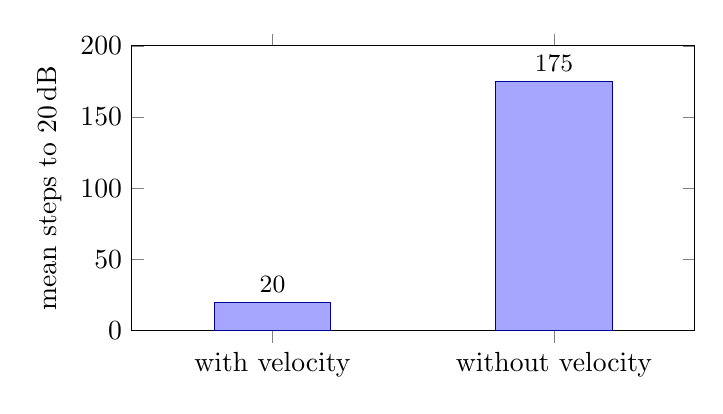
\begin{tikzpicture}
    \begin{axis}[
        ybar, width=0.72\textwidth, height=5.2cm,
        ylabel={mean steps to $20$\,dB}, ymin=0, ymax=200,
        symbolic x coords={with velocity, without velocity},
        xtick=data, bar width=42pt,
        nodes near coords, every node near coord/.append style={font=\small},
        enlarge x limits=0.5,
    ]
    \addplot[fill=blue!35, draw=blue!60!black] coordinates {(with velocity,20) (without velocity,175)};
    \end{axis}
    \end{tikzpicture}
    \caption{Mean tracking steps required to reach a $20$\,dB object-PSNR target, with
    and without linear velocity prediction (40-frame sequence). Velocity prediction
    cuts the per-frame step count by roughly $89\%$.}
    \label{fig:velocity-bars}
\end{figure}

\subsection{Frustum Clamping}
\label{sec:results-snap}

Per-frame hull snapping is compared against the milder velocity-gating fallback over a
16-frame tracking run (Table~\ref{tab:snap}). The comparison is designed to expose the
runaway and left-behind failure modes of Section~\ref{sec:velocity}: gating only stops
strays from coasting, whereas snapping actively reclaims them. Snapping keeps the
subject markedly more complete and higher in quality, with mean object coverage rising
from $0.893$ to $0.971$ and mean object PSNR from $13.24$ to $14.27$\,dB. It also keeps
the cloud tighter, with the maximum primitive radius from the centre falling from
$0.24$ to $0.19$ (a direct measure of how far runaways have escaped).

The most telling statistic is not the mean but the \emph{trend}. Under gating, object
coverage degrades from $1.00$ at the first tracking frame to $0.78$ by the sixteenth as
primitives are progressively left behind, whereas under snapping it holds at $0.94$. By
the last frame snapping leads by roughly $1.5$\,dB and $0.16$ in coverage, and the gap
widens monotonically over the sequence. A widening gap is the signature of a mechanism
that counteracts a \emph{cumulative} degradation rather than merely a constant offset:
each frame, snapping undoes the strays that gating would have allowed to accumulate, so
its advantage compounds. This is exactly the behaviour predicted by the runaway
analysis, in which un-reclaimed primitives are lost permanently and never replaced under
the fixed count.

\begin{table}[!ht]
    \centering
    \begin{tabular}{lccc}
        \toprule
        & mean object coverage & mean object PSNR & final cloud radius \\
        \midrule
        velocity gating          & $0.893$ ($1.00\!\to\!0.78$) & $13.24$\,dB ($\to 10.6$) & $0.24$ \\
        hull snapping \emph{(default)} & $\mathbf{0.971}$ ($1.00\!\to\!0.94$) & $\mathbf{14.27}$\,dB ($\to 12.1$) & $\mathbf{0.19}$ \\
        \bottomrule
    \end{tabular}
    \caption{Frustum clamping over a 16-frame tracking run. Parenthetical values show
    the first-to-last-frame trend. Snapping reclaims strays instead of leaving them
    behind, holding coverage and quality.}
    \label{tab:snap}
\end{table}

\subsection{Foreground Masking}
\label{sec:results-masking}

The silhouette supervision of Section~\ref{sec:masking} is evaluated by tracking the
mean rendered opacity that leaks into the clearly-background region over a 16-frame run,
a direct measure of the background drift the mechanism is meant to suppress
(Table~\ref{tab:masking}). With the naive full-image loss, the leak grows by roughly
two orders of magnitude across the sequence, from $0.0001$ at the first frame to
$0.0127$ at the last, as dead primitives accumulate in empty space, and object coverage
degrades to about $0.82$. With the masked loss and silhouette supervision the leak stays
flat and low (mean $0.0020$, a threefold reduction) and the subject stays solid, holding
$0.86$ to $0.95$ coverage. Crucially, it is not only the mean leak that improves but its
\emph{growth}. The drift that compounds frame over frame under the full-image loss is
essentially eliminated, which is what matters for a long capture.

The same experiment validates the decision to leave opacity trainable. Additionally
freezing opacity makes the leak about sixfold worse than the default, rising to $0.044$,
for exactly the reason given in Section~\ref{sec:masking}. A primitive pushed into the
background then has neither a photometric pull-back (the loss is masked away there) nor
the ability to fade out (opacity is frozen), so it remains stuck bright and opaque
off-object. Keeping opacity free is therefore what allows the silhouette term to fade
strays away, and the measurements confirm that the count- and colour-freezing
philosophy should not be extended to opacity.

\begin{table}[!ht]
    \centering
    \begin{tabular}{lccc}
        \toprule
        & mean background leak & leak trend (16 frames) & object coverage \\
        \midrule
        full-image loss              & $0.0059$ & grows $\sim\!100\times$ ($0.0001\!\to\!0.0127$) & degrades to $\sim\!0.82$ \\
        masked $+$ silhouette \emph{(default)} & $\mathbf{0.0020}$ & flat \& low ($\le 0.0033$) & holds $0.86$ to $0.95$ \\
        freeze opacity \& colour     & $0.0123$ & grows worst ($\to 0.044$) & $0.888$ \\
        \bottomrule
    \end{tabular}
    \caption{Background-drift suppression. Masking the photometric loss and supervising
    the silhouette suppresses background fitting and, more importantly, eliminates its
    frame-over-frame growth.}
    \label{tab:masking}
\end{table}

\subsection{Temporal Compression}
\label{sec:results-compression}

The compressor is evaluated on a 123-frame sequence of $4256$ primitives ($35.6$\,MB
raw) by sweeping the single quality knob $q$ of Eq.~\eqref{eq:choosek} and measuring
both the on-disk compression ratio and the render PSNR of the reconstructed clouds
against the originals (Table~\ref{tab:compression}, Figure~\ref{fig:rate-distortion}).
At the default $q = 0.999$ the sequence compresses by $9.6\times$ at $30.1$\,dB,
already roughly twice the $5\times$ target at this quality, and the operating point
moves smoothly from $6.8\times$ at $37.9$\,dB down to $41.6\times$ at $25.1$\,dB as $q$
is lowered. The rate-distortion curve is steep at the high-fidelity end, meaning a
small concession in PSNR buys a large reduction in size, and flattens toward the
aggressive end, the usual diminishing return of lossy compression.

Two structural facts explain the favourable numbers. First, colours and normals are
\emph{exactly} lossless, handled by the constant and zero modes rather than by
truncation, so all error is confined to geometry, where the position error is under
$1\%$ of the scene span. Second, the per-attribute coefficient budget confirms the
motivation for the DCT: the smooth position channels are captured by only about $15$,
$19$, and $7$ coefficients in $x$, $y$, and $z$ respectively, whereas the noisier
opacity and quaternion channels consume the most coefficients and hit the cap. This
points directly at where further gains lie, since lowering the cap on the noisy channels
costs little fidelity, and confirms that the smooth, predictable motion the velocity
model exploits is also what the compressor exploits, from the opposite direction.

\begin{table}[!ht]
    \centering
    \begin{tabular}{lcc}
        \toprule
        quality $q$ & compression ratio & render PSNR vs.\ original \\
        \midrule
        $0.98$  & $41.6\times$ & $25.1$\,dB \\
        $0.99$  & $25.7\times$ & $25.6$\,dB \\
        $0.995$ & $15.9\times$ & $26.4$\,dB \\
        $0.999$ \emph{(default)} & $\mathbf{9.6\times}$ & $\mathbf{30.1}$\,dB \\
        $0.9999$ & $6.8\times$ & $37.9$\,dB \\
        \bottomrule
    \end{tabular}
    \caption{Temporal compression rate-distortion on a 123-frame, 4256-primitive
    sequence. A single quality knob $q$ trades ratio against fidelity.}
    \label{tab:compression}
\end{table}

\begin{figure}[!ht]
    \centering
    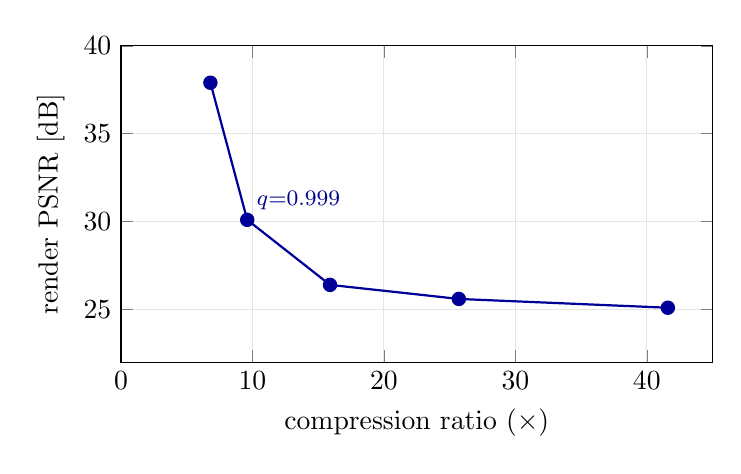
\begin{tikzpicture}
    \begin{axis}[
        width=0.75\textwidth, height=5.6cm,
        xlabel={compression ratio ($\times$)}, ylabel={render PSNR [dB]},
        xmin=0, xmax=45, ymin=22, ymax=40,
        grid=both, grid style={gray!20},
        mark size=2.2pt,
    ]
    \addplot[blue!60!black, thick, mark=*] coordinates {
        (6.8,37.9) (9.6,30.1) (15.9,26.4) (25.7,25.6) (41.6,25.1)
    };
    \node[anchor=south west, font=\footnotesize, blue!55!black] at (axis cs:9.6,30.1) {$q{=}0.999$};
    \end{axis}
    \end{tikzpicture}
    \caption{Rate-distortion curve of the temporal compressor. The default operating
    point ($q = 0.999$, $9.6\times$, $30.1$\,dB) is marked; fidelity rises steeply as
    the ratio is relaxed.}
    \label{fig:rate-distortion}
\end{figure}

\subsection{Summary}
\label{sec:results-summary}

Taken together, the measurements support the three design claims of
Section~\ref{sec:overview}. Temporal coherence and bounded cost follow from the
constant-count, frozen-colour tracking regime, which both the merge renderer and the
temporal compressor exploit from opposite ends: the renderer composites a fixed-size
cloud per frame with zero re-upload, and the compressor reaches roughly $10\times$ at
$30$\,dB by treating each primitive's trajectory as a smooth, individually-truncated
time series. The separation of motion from appearance is enforced jointly by the frozen
colours, the silhouette supervision that prevents background drift, and the frustum
snapping that reclaims strays, together holding object coverage near $0.97$ where the
unconstrained baseline degrades below $0.80$. Velocity prediction makes the regime
efficient, cutting per-frame tracking by roughly $89\%$ while improving final quality.
These measurements are accompanied by qualitative renders, collected in the following
figures: per-frame montages of the moving subject, the composited scene in the merge
renderer, and the displacement-coloured emergent partition.

\begin{figure}[!ht]
    \begin{center}
        \fbox{\parbox{0.85\linewidth}{\vspace{3.5cm}\centering\emph{[Placeholder:
        montage of reconstructed frames $t = 0, 10, \dots$ of the moving subject, with
        ground truth alongside, showing temporal consistency.]}\vspace{3.5cm}}}
    \end{center}
    \caption{Qualitative temporal consistency of the dynamic reconstruction.}
    \label{fig:qual-temporal}
\end{figure}

\begin{figure}[!ht]
    \begin{center}
        \fbox{\parbox{0.85\linewidth}{\vspace{3.5cm}\centering\emph{[Placeholder:
        screenshot of the merge renderer compositing the static background with the
        dynamic foreground, with the playback controls visible.]}\vspace{3.5cm}}}
    \end{center}
    \caption{The static background and dynamic foreground composited in the merge
    renderer.}
    \label{fig:qual-merge}
\end{figure}

\begin{figure}[!ht]
    \begin{center}
        \fbox{\parbox{0.85\linewidth}{\vspace{3.5cm}\centering\emph{[Placeholder:
        emergent partition, every primitive coloured by the magnitude of its
        cumulative displacement $D_i$, so the stationary background appears cold and the
        moving subject warm, recovering a segmentation without any mask.]}\vspace{3.5cm}}}
    \end{center}
    \caption{The emergent static-dynamic partition, recovered by thresholding
    cumulative per-primitive displacement.}
    \label{fig:qual-partition}
\end{figure}
